\documentclass[aspectratio=169,xcolor=dvipsnames]{beamer}
\usetheme{SimplePlus}

% Math
\usepackage{nicefrac}

% Tipography stuff
\usepackage{booktabs} % Allows the use of \toprule, \midrule and \bottomrule in tables
\usepackage[english]{babel}
\usepackage{csquotes}
\usepackage{microtype}
\usepackage{pdfpages}
\usepackage{fontawesome5}
\usepackage{soul}
\usepackage{euler}
\usepackage{algorithm2e}
\usepackage{animate}
\usepackage{ifthen}

% Bibliography
\usepackage[giveninits,style=authoryear-comp,backend=biber]{biblatex}
\addbibresource{../fracbiblio.bib}
\newcommand\unnumbered{\setbeamertemplate{footline}{}}%\addtocounter{framenumber}{-1}
\renewcommand*{\bibfont}{\normalfont\small}

% Figures
\usepackage{tikz,pgfplots}
\usetikzlibrary{calc,arrows,patterns,matrix,external}
\usepackage{subfig}
\usepackage{graphicx} % Allows including images
\usepackage[american]{circuitikz}
\usepackage{tikz-network}
\tikzexternalize[prefix=Figures/] % activate and define figures/ as cache folder

% Links
\usepackage{hyperref}
\hypersetup{colorlinks,linkcolor=,urlcolor=MidnightBlue}

% Code
\usepackage{minted}

% Block matrices
\newcommand{\bigzero}{\mbox{\normalfont\Large\bfseries 0}}
\newcommand{\rvline}{\hspace*{-\arraycolsep}\vline\hspace*{-\arraycolsep}}
\newcommand{\R}{\mathbb{R}}
\newcommand{\bone}{{\bf 1}}
\newcommand{\evec}{{\bf e}}
\newcommand{\dvec}{{\bf d}}
\newcommand{\xvec}{{\bf x}}
\newcommand{\yvec}{{\bf y}}
\newcommand{\qvec}{{\bf q}}
\newcommand{\svec}{{\bf s}}
\newcommand{\pvec}{{\bf p}}
\newcommand{\tvec}{{\bf t}}
\definecolor{Ao}{rgb}{0.0, 0.5, 0.0}


\author{Fabio Durastante}
\title{An introduction to fractional calculus}
\subtitle{Fundamental ideas and numerics}
\institute{Università di Pisa\\\href{mailto:fabio.durastante@unipi.it}{\faEnvelope\;fabio.durastante@unipi.it}\\\href{https://fdurastante.github.io}{\faFirefox\;fdurastante.github.io}}
\date{September, 2022}

\newcommand{\de}{{\rm d}}


\begin{document}

{\unnumbered
\begin{frame}[t,plain,noframenumbering]
\titlepage
\vspace{-4em}
\includegraphics[width=2cm]{frame.png}
\end{frame}
}

\section{Fractional Diffusion Equation}

\begin{frame}{Fractional Diffusion Equation}

Starting from the past$\ldots$

\begin{itemize}
	\item[\faMemory]<2-> We have seen in \textbf{Lecture 5} that there is a connection between \alert<2>{\textbf{diffusion equations}} and \alert<2>{\textbf{random walks}},
	\item[\faLightbulb]<3-> Given a \textbf{particle} we can act either on the \faWalking\,\alert<3>{jump length} or on the \faClock\,\alert<3>{waiting time}. 
\end{itemize}

\onslide<4->{The \alert{\textbf{C}}ontinuous \alert{\textbf{T}}ime \alert{\textbf{R}}andom \alert{\textbf{W}}alk model (CTRW):
\begin{itemize}
	\item[\faLightbulb] Both the \textbf{length of a given jump}, and the \textbf{waiting time}
	elapsing between two successive jumps are drawn from a pdf $\psi(x,t)$
	\item[\faWalking]<5-> $\displaystyle \lambda(x) = \int_{0}^{+\infty} \psi(x,y)\,\textrm{d}t,$ \emph{jump length},
	\begin{onlyenv}<5>
		\begin{exampleblock}{Jump length}
			$\lambda(x) \textrm{d}x$ produces the probability for a jump length in the interval $(x,x+\textrm{d}x)$.
		\end{exampleblock}
	\end{onlyenv}
	\item[\faClock]<6-> $\displaystyle w(t) = \int_{-\infty}^{+\infty} \psi(x,t)\,\textrm{d}x,$ \emph{waiting time},
	\begin{onlyenv}<6>
		\begin{exampleblock}{Waiting time}
			$w(t) \textrm{d}t$ produces the probability for a waiting time in the interval $(t,t+\textrm{d}t)$.
		\end{exampleblock}
	\end{onlyenv}
	\only<7->{
		\item If the jump length and
		waiting time are \textbf{independent random variables} then: \[\psi(x,t) = w(t)\lambda(x).\]
	}
\end{itemize}}

\end{frame}


\begin{frame}{Characterization of CTRW}
	To categorise different CTRW one can look at the quantities
	\[
	T = \int_{0}^{+\infty} t w(t)\,\textrm{d}t, \text{ (Characteristic waiting time)},
	\]
	and 
	\[
	\Sigma^2 = \int_{-\infty}^{+\infty} x^2\lambda(x)\,\textrm{d}x\, \text{ (Jump length variance)},
	\]
	specifically, are they \textbf{finite}? Do they \textbf{diverge}?
	
	\onslide<2->{
		The \alert{master} (Langevin) \alert{equation} for this process is then given by
		\[
		\alert<3>{\eta(x,t)} = \int_{-\infty}^{+\infty} \textrm{d}x' \int_{0}^{+\infty} \textrm{d}t'\,\alert<4>{\eta(x',t')} \psi(x-x',t-t') + \delta(x)\delta(t),
		\]
		\only<3->{Pdf of having arrived at position $x$ at time $t$ -- $\eta(x,t)$ --}\only<4->{ having just arrived at $x'$ at time $t'$ -- $\eta(x',t')$ --}\only<5->{ with initial condition $\delta(x)$.}
	}
	
\end{frame}

\begin{frame}{Characterization of CTRW}
	Then if we use 
	\[
	\eta(x,t) = \int_{-\infty}^{+\infty} \textrm{d}x' \int_{0}^{+\infty} \textrm{d}t'\,\eta(x',t') \psi(x-x',t-t') + \delta(x)\delta(t),
	\]
	we can write the pdf of being in $x$ at time $t$ as
	\[
	W(x,t) = \int_{0}^{t} \eta(x,t') \Psi(t-t'),\textrm{d}t, \qquad \Psi(t) = 1 - \int_{0}^{t} w(t')\,\textrm{d}t',
	\]
	where the latter is the cumulative probability assigned to the probability of \alert{no jump event} during the time interval  $t-t'$.
	\begin{onlyenv}<1>
	\begin{alertblock}{Fact I - Ordinary Diffusion}
		If both $T$ and $\Sigma^2$ are finite the long-time limit corresponds to Brownian motion, e.g., $w(t) = \tau^{-1} exp(-\nicefrac{t}{\tau})$, $T = \tau$, $\lambda(x) = (4\pi \sigma^2)^{-\nicefrac{1}{2}} \exp(-\nicefrac{x^2}{4\sigma^2})$, $\Sigma^2 = 2 \sigma^2$, we recover the standard diffusion equation.
	\end{alertblock}
	\end{onlyenv}
	\begin{onlyenv}<2>
	\begin{alertblock}{Fact II - Subdifussion}
		The \textbf{characteristic waiting time} $T = \int_{0}^{+\infty} t w(t)\,\textrm{d}t$ \textbf{diverges}, but the jump length variance $\Sigma^2 = \int_{-\infty}^{+\infty} x^2\lambda(x)\,\textrm{d}x$ is finite, we obtain a \textbf{subdiffusive process}. Particles make long rests.
	\end{alertblock}
	\end{onlyenv}
\end{frame}

\begin{frame}{Long jumps: L\'evy Flights}
	What if we take a \textbf{finite waiting time} and a \textbf{diverging jump length}?
	\begin{itemize}
		\item[\faClock]<2-> Poissonian waiting time, \onslide<5->{\textbf{Rmk:} $T$ is \textbf{finite} and so the process is \textbf{Markovian}!}
		\item[\faWalking]<3-> L\'evy distribution for the jump length
		\[
		\lambda(k) = \exp(-\sigma^\mu |k|^\mu) \sim 1 - \sigma^\mu |k|^\mu, 
		\]
	\end{itemize}\vspace{-1em}
	\begin{block}<4->{Asymptotic}
	For $|x| \gg \sigma$, $1 < \mu < 2$ $\Rightarrow$ $\lambda(x) \sim A_\mu \sigma^{-\mu} |x|^{-1-\mu}$.
	\end{block}
	\begin{itemize}
		\item<6-> In the \alert{Fourier-Laplace space} we get
		\[
		W(k,u) = \frac{1}{u + K^\mu |k|^\mu},
		\]
		\item<7-> then after a (double) inversion
		\only<7>{\[\frac{\partial W}{\partial t} = K^{\mu} \cdot \frac{1}{\Gamma(1-\mu)} \frac{\textrm{d}}{\textrm{d}x}\int_{-\infty}^{x} W(\xi,t){(x-\xi)^\alpha}\,\mathrm{d}\xi, \quad K = \frac{\sigma^\mu}{\tau} \]}
		\only<8>{\[\frac{\partial W}{\partial t} = K^{\mu}\, {}^{RL}D_{(-\infty,x)}^\mu W(x,t), \quad K = \frac{\sigma^\mu}{\tau} \]}
	\end{itemize}
\end{frame}

\begin{frame}[fragile]{Brownian jumps vs L\'evy Flights}
\vspace{-2em}
\begin{columns}[t]
\begin{column}{0.35\columnwidth}
\begin{center}
	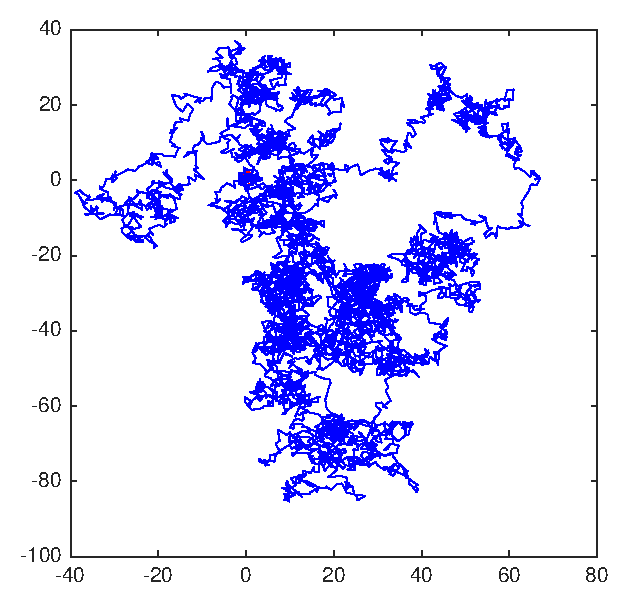
\includegraphics[height=11em]{Figures/brown.eps}
\end{center}
\definecolor{bg}{rgb}{0.95,0.95,0.95}\vspace{-1.6em}
\begin{minted}[bgcolor=bg,fontsize=\small,breaklines]{matlab}
%% Brownian motion
N = 7000;
x = cumsum(randn(N,1));
y = cumsum(randn(N,1));
\end{minted}
\end{column}
\begin{column}{0.62\columnwidth}
\begin{center}
	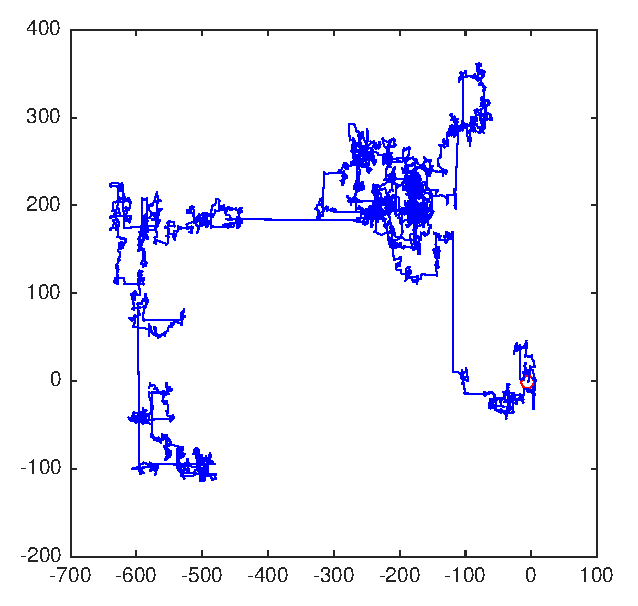
\includegraphics[height=11em]{Figures/levy.eps}
\end{center}
\definecolor{bg}{rgb}{0.95,0.95,0.95}\vspace{-1.6em}
\begin{minted}[bgcolor=bg,fontsize=\small,breaklines]{matlab}
%% Levy distribution
N = 7000;
pd_levy = makedist('Stable','alpha',1.5, 'beta',0,'gam',1, 'delta',0);
xl = cumsum(random(pd_levy,N,1));
yl = cumsum(random(pd_levy,N,1));
\end{minted}
\end{column}
\end{columns}	

\end{frame}

\subsection{The (Space) Fractional Diffusion Equations}

\begin{frame}{The (Space) Fractional Diffusion Equations}
We want to solve our problem in a \textbf{domain of finite size}, therefore we have to move the lower and upper bounds of the Riemann-Liouville integral to a finite domain size and \textbf{select} some \textbf{\alert{boundary conditions}}.

\begin{block}<2->{Absorbing boundary conditions (Dirichlet)}
A common choice is given by: $W(x_l,t) = W(x_r,T) \equiv 0$
\end{block}

\onslide<3->{They can be justified in various way
\begin{itemize}
	\item<4->[\faFile*] Variational formulation from a generalized \emph{Fickian} law \parencite{MR3378843},
	\item<5->[\faFile*] Lyapunov inequality \parencite{MR3124347}.
\end{itemize}
}
\onslide<6>{
\begin{equation}\label{eq:fde1}
	\begin{cases}\frac{\partial W}{\partial t} = \theta\,{}^{RL}D_{[0,x]}^\alpha W(x,t) + (1-\theta) {}^{RL}D_{[x,1]}^\alpha W(x,t), \qquad \theta \in [0,1] \tag{FDE\textsubscript{1}},\\
	W(0,t) = W(1,t) = 0,\\
	W(x,t) = W_0(x).	
	\end{cases}
\end{equation}
}

\end{frame}

\section{Finite Difference Approaches to Riemann--Liouville}

\begin{frame}{Finite Difference Approaches to Riemann--Liouville}
	
The \textbf{first approach} we want to discuss is \alert{\textbf{finite differences}}, thus how can we discretize the Riemann-Liouville operators?

\begin{alertblock}<2->{Back to the basics}
\begin{enumerate}
	\item<2-> First derivative
	\[
	\frac{\mathrm{d} f}{\mathrm{d}x} = \lim_{h \rightarrow 0} \frac{f(x)-f(x-h)}{h},
	\]
	\item<3-> $n$th derivative
	\[
	\frac{\mathrm{d}^n f}{\mathrm{d}x^n} = \lim_{h \rightarrow 0} \frac{\Delta^n f(x)}{h}, \quad \Delta^n f(x) = \sum_{j=0}^{n}\binom{n}{j}(-1)^j f(x-jh).
	\]
\end{enumerate}
\end{alertblock}

\begin{itemize}
	\item[\faLightbulb]<4-> Let's use again our favourite trick and replace $n \in \mathbb{N}$ with $\alpha \in \mathbb{R}$!
\end{itemize}

\end{frame}

\begin{frame}{The Gr\"unwald--Letnikov Fractional Derivative}

\begin{exampleblock}{The Gr\"unwald--Letnikov Fractional Derivative \parencite{grunwald1867uber,letnikov1868theory}}
Given $\mathbb{R} \ni \alpha > 0$ define the Gr\"unwald--Letnikov fractional derivative of a function $f(x)$~as
\[
{}^{GL}D^\alpha f = \lim_{h \rightarrow 0} \frac{\Delta^\alpha f(x)}{h}, \quad \Delta^\alpha f(x) = \sum_{j=0}^{+\infty}\binom{\alpha}{j}(-1)^j f(x-jh), \quad \binom{\alpha}{j} = \frac{\Gamma(\alpha+1)}{j! \Gamma(\alpha-j+1)}.
\]
\end{exampleblock}

\begin{itemize}
	\item[\faQuestionCircle]<2-> For what functions $f$ does it make sense?
	\item[\faQuestionCircle]<3-> How is it related to the Riemann-Liouville (and henceforth to the Caputo) fractional derivative?
	\item[\faLightbulb]<4-> If we can find an easy relation with the Riemann-Liouville derivative we can \textbf{use it to discretize} by truncating $\Delta^\alpha$ to a given $N$.
\end{itemize}

\end{frame}

\begin{frame}{The Gr\"unwald--Letnikov Fractional Derivative}

Let us collect the ingredients we need.

\begin{itemize}
	\item[\faInbox] The \alert{binomial series} 
	\[
	(1+z)^\alpha = \sum_{j=0}^{+\infty} \binom{\alpha}{j} z^j,
	\]
	converges for any $z \in \mathbb{C}$ with $|z| \leq 1$ and any $\alpha > 0$,
	\item[\faInbox] The series
	\[
	\sum_{j=0}^{+\infty}\left\lvert \binom{\alpha}{j} (-1)^j \right\rvert < +\infty,
	\]
	converges, since $(1+(-1))^\alpha = 0$.
	\item[$\Rightarrow$] If we take $f$ to be bounded then ${}^{GL}D^\alpha f$ exists.
\end{itemize}

\end{frame}

\begin{frame}{The Gr\"unwald--Letnikov Fractional Derivative}
	
Let us take the Fourier transform of $\Delta^\alpha f(x)$
\[
\begin{split}
\int e^{-ikx} \sum_{j=0}^{+\infty} \binom{\alpha}{j} (-1)^j f(x-jh)\,\mathrm{d}x \only<1>{= & \sum_{j=0}^{+\infty} \binom{\alpha}{j}(-1)^j \int e^{-ikx}f(x-jh)\,\mathrm{d}x \\
= & \sum_{j=0}^{\infty} \binom{\alpha}{j}(-1)^j e^{-ikjh}\hat{f}(k) \\}
= & (1-e^{-ikh})^\alpha \hat{f}(k).
\end{split}
\]
\begin{itemize}
	\item[\faBook] We are using the \textbf{uniform convergence} of the series $\Delta^\alpha f(x)$,
	\item[\faExclamationCircle] furthermore we are \textbf{requiring} that each term is integrable.
\end{itemize}
\begin{onlyenv}<2->
If $k \neq 0$ then the Fourier transform of the GL derivative operator is given by
\[
h^{-\alpha}(ikh)^{\alpha} \left( \frac{1-e^{-ikh}}{ikh} \right) \hat{f}(k) \rightarrow (ik)^\alpha \hat{f}(k), \text{ for } h \rightarrow 0.
\]
The same holds by direct computation for $k=0$.
\begin{itemize}
\item[$\Rightarrow$]<3-> The Fourier transform \textbf{converges} \textbf{pointwise} to the same \textbf{Fourier} \textbf{transform} of the \textbf{Riemann-Liouville} derivative (we are also using the \alert{continuity Theorem} of Fourier transform.)
\end{itemize}
\end{onlyenv}
	
\end{frame}

\begin{frame}{The Gr\"unwald--Letnikov Fractional Derivative}
What is the connection then? 
\begin{enumerate}
	\item<2-> Let us look better into the \emph{weights}
	\[
	\begin{split}
	g_j^{(\alpha)} \triangleq  (-1)^j \binom{\alpha}{j} \only<2>{= & \frac{(-1)^j \Gamma(\alpha+1)}{\Gamma(j+1)\Gamma(\alpha-j+1)} = \\
	= & \frac{(-1)^j\alpha(\alpha-1)\cdots(\alpha-j+1)}{\Gamma(j+1)} \\
	\text{\scriptsize Distribute $(-1)^j \rightarrow$} = & \frac{(-\alpha)(1-\alpha)\cdot(j-1-\alpha)}{\Gamma(j+1)} \\}
	= & \frac{-\alpha \Gamma(j-\alpha)}{\Gamma(j+1)\Gamma(1-\alpha)}
	\end{split}
	\]
	\item<3-> Using $\Gamma(x+1)=x\Gamma(x)$ and $\Gamma(x+1) \sim \sqrt{2\pi x} x^x e^{-x}$ for $x\rightarrow+\infty$
	\[
	\begin{split}
	g_j^{(\alpha)} \sim & \only<3>{ \frac{-\alpha}{\Gamma(1-\alpha)} \frac{\sqrt{2\pi(j-\alpha-1)}(j-\alpha-1)^{j-\alpha-1} e^{-(j-\alpha-1)}}{\sqrt{2\pi j} j^j e^{-j}} \\
	= & \frac{-\alpha}{\Gamma(1-\alpha)} \underbrace{\sqrt{\frac{j-\alpha-1}{j}}}_{\rightarrow 1} \underbrace{\left( \frac{j-\alpha-1}{j} \right)^{j-\alpha-1}}_{\rightarrow e^{-(\alpha+1)}} j^{-\alpha-1}e^{\alpha+1}}
	\only<4->{ \frac{-\alpha}{\Gamma(1-\alpha)}} j^{-\alpha-1} \qquad j \rightarrow +\infty.
	\end{split}
	\]
	\item<5-> Since $g_0^{(\alpha)} = 1$ we write the quotient
	\[
	\frac{\Delta^\alpha f(x)}{\Delta x^\alpha} = (\Delta x)^{-\alpha} \left[ f(x) + \sum_{j=1}^{+\infty} g_j^{(\alpha)} f(x-j\Delta x) \right]
	\]
\end{enumerate}
\end{frame}

\begin{frame}{The Gr\"unwald--Letnikov Fractional Derivative}
	What is the connection then? 
\begin{enumerate}
	\setcounter{enumi}{2}
	\item Since $g_0^{(\alpha)} = 1$ we write the quotient
	\[
	\frac{\Delta^\alpha f(x)}{\Delta x^\alpha} = (\Delta x)^{-\alpha} \left[ f(x) + \sum_{j=1}^{+\infty} g_j^{(\alpha)} f(x-j\Delta x) \right]
	\]
	\item<2-> $\sum_{j=0}^{+\infty}w_j = 0$. Then $g_j^{(\alpha)} < 0$ for all $j \geq 1$ and thus $\sum_{j=1}^{+\infty} g_j^{(\alpha)} = -1$. We \textbf{define} $b_j^{(\alpha)} = - w^{(\alpha)}_j$ for $j \geq 1$, so that
	\[
	b_j \sim \frac{\alpha}{\Gamma(1-\alpha)}j^{-\alpha-1} \text{ for } j \rightarrow +\infty, \qquad \sum_{j=1}^{+\infty} b_j = 1.
	\]
\end{enumerate}
\end{frame}

\begin{frame}{The Gr\"unwald--Letnikov Fractional Derivative}
Then we take $0 < \alpha < 1$
\[
\begin{split}
\frac{\Delta^\alpha f(x)}{\Delta x^\alpha} = & (\Delta x)^{-\alpha} \sum_{j=1}^{+\infty}[f(x) - f(x-j\Delta x)] b_j \\
\approx & \sum_{j=1}^{+\infty} [f(x) - f(x-j\Delta x)] \frac{\alpha}{\Gamma(1-\alpha)} (j\Delta x)^{-\alpha-1} \Delta x \\
\approx & \int_{0}^{+\infty} [f(x)-f(x-y)] \frac{\alpha}{\Gamma(1-\alpha)} y^{-\alpha-1}\,\mathrm{d}y
\end{split}
\]
\begin{itemize}
	\item<2-> Integrate by parts with $u = f(x) - f(x-y)$\only<4>{$\ldots$ and when you swap the integral and the derivative}
	\[
	\only<2-3>{\only<3>{ {}^{CA} D_{[0,+\infty]}^\alpha f(x) =   }\frac{1}{\Gamma(1-\alpha)} \int_{0}^{+\infty} f'(x-y)y^{-\alpha}\,\mathrm{d}y = \frac{1}{\Gamma(1-\alpha)}\int_{0}^{+\infty} \frac{\mathrm{d}}{\mathrm{d}x} f(x-y) y^{-\alpha}\,\mathrm{d}y}
	\only<4>{
	{}^{RL} D_{[0,+\infty]}^\alpha = \frac{1}{\Gamma(1-\alpha)} \frac{\mathrm{d}}{\mathrm{d}x} \int_{0}^{+\infty} f(x-y) y^{-\alpha}\,\mathrm{d}y.
	}
	\]
\end{itemize}
\end{frame}

\begin{frame}{The Gr\"unwald--Letnikov Fractional Derivative}
Let us move everything to a fixed interval $[a,b]$.
\begin{exampleblock}{Gr\"unwald--Letnikov \emph{revisited}}
Let $\alpha > 0$, $f \in \mathcal{C}^{\lceil \alpha \rceil}([a,b])$, $a < x \leq b$, then
\[
{}^{GL}D_{[a,x]}f(x) = \lim_{N \rightarrow + \infty} \frac{\Delta_{h_N}^\alpha f(x)}{h_N^\alpha} = \lim_{N \rightarrow + \infty} \frac{1}{h_N^\alpha}\sum_{k=0}^{N} (-1)^k \binom{\alpha}{k} f(x - k h_N),
\]
with $h_N = (x-a)/N$.
\end{exampleblock}

\alert{\faEye} In the definition we have implicitly extended $f$ (with an abuse of notation) in such a way that
\[
f : (-\infty,b] \rightarrow \mathbb{R}, \qquad x \mapsto \begin{cases}
f(x), & \text{ if } x \in [a,b],\\
0, & \text{ if } x \in (-\infty,a).
\end{cases}
\]
	
\end{frame}

\begin{frame}[fragile]{Computing the coefficients}

We can compute $N+1$ $g_j^{(\alpha)}$ coefficients in $3N+1$ flops by using the recurrence relation
\[
g_j^{(\alpha)} = \left( 1  - \frac{\alpha+1}{j} \right) g_{j-1}^\alpha, \quad g_0 = 1.
\]
\begin{columns}
\begin{column}{0.55\columnwidth}
In a line of code
\definecolor{bg}{rgb}{0.95,0.95,0.95}
\begin{minted}[bgcolor=bg,fontsize=\small,breaklines]{matlab}
function [g] = gl(n,alpha)
%GL Produces the N+1 Grunwald-Letnikov coefficients for a given alpha
g = cumprod([1, 1 - ((alpha+1) ./ (1:n))]);
end
\end{minted}
\end{column}
\begin{column}{0.45\columnwidth}
\centering
%% This file was created by matlab2tikz.
%
%The latest updates can be retrieved from
%  http://www.mathworks.com/matlabcentral/fileexchange/22022-matlab2tikz-matlab2tikz
%where you can also make suggestions and rate matlab2tikz.
%
\definecolor{mycolor1}{rgb}{0.00000,0.44700,0.74100}%
\definecolor{mycolor2}{rgb}{0.92900,0.69400,0.12500}%
\definecolor{mycolor3}{rgb}{0.46600,0.67400,0.18800}%
%
\begin{tikzpicture}

\begin{axis}[%
width=0.6\columnwidth,
height=0.6\columnwidth,
at={(0.758in,0.481in)},
scale only axis,
xmode=log,
xmin=1,
xmax=500,
xminorticks=true,
ymode=log,
ymin=8.69668964364581e-09,
ymax=1.8,
yminorticks=true,
axis background/.style={fill=white},
legend style={legend cell align=left, align=left, draw=none, fill=none}
]
\addplot [color=mycolor1, line width=2.0pt, only marks, mark=o, mark options={solid, mycolor1}]
  table[row sep=crcr]{%
0	1\\
10	0.001496322048\\
20	0.000302980825332931\\
30	0.000121334787852135\\
40	6.37058571319524e-05\\
50	3.87289678320561e-05\\
60	2.58158074015452e-05\\
70	1.83321528132578e-05\\
80	1.36330085288554e-05\\
90	1.05014470948618e-05\\
100	8.31645016375941e-06\\
110	6.73514929930017e-06\\
120	5.55614750255491e-06\\
130	4.65507073274176e-06\\
140	3.95186706490171e-06\\
150	3.39318936411088e-06\\
160	2.94241740988927e-06\\
170	2.57376207124882e-06\\
180	2.26865233870373e-06\\
190	2.01345014148621e-06\\
200	1.79796431795493e-06\\
210	1.61446025771274e-06\\
220	1.45698529027345e-06\\
230	1.32090005295272e-06\\
240	1.20254713634538e-06\\
250	1.09901300620354e-06\\
260	1.00795442669456e-06\\
270	9.2747020709511e-07\\
280	8.56005266868795e-07\\
290	7.92278058804823e-07\\
300	7.35225085678139e-07\\
310	6.83958071029497e-07\\
320	6.37730598409415e-07\\
330	5.9591190633955e-07\\
340	5.57966141658716e-07\\
350	5.23435812892549e-07\\
360	4.91928501839234e-07\\
370	4.63106122185075e-07\\
380	4.36676183601537e-07\\
390	4.12384645688165e-07\\
400	3.90010040383013e-07\\
410	3.69358612591942e-07\\
420	3.50260282874737e-07\\
430	3.32565277450256e-07\\
440	3.16141302726627e-07\\
450	3.00871166355927e-07\\
460	2.86650766175399e-07\\
470	2.73387383607858e-07\\
480	2.60998230109867e-07\\
490	2.49409204799489e-07\\
500	2.38553829013523e-07\\
};
\addlegendentry{$\alpha\text{=1.1}$}

\addplot [color=black, dashed, line width=2.0pt]
  table[row sep=crcr]{%
80	1.34083269433444e-05\\
81	1.30468455421953e-05\\
82	1.26993673840321e-05\\
83	1.23651890103417e-05\\
84	1.20436501973314e-05\\
85	1.17341308247606e-05\\
86	1.14360480050724e-05\\
87	1.11488534484594e-05\\
88	1.0872031042033e-05\\
89	1.06050946235021e-05\\
90	1.03475859317599e-05\\
91	1.00990727185435e-05\\
92	9.85914700690485e-06\\
93	9.62742348363169e-06\\
94	9.40353801401038e-06\\
95	9.18714626843659e-06\\
96	8.97792245138133e-06\\
97	8.77555812411334e-06\\
98	8.57976111338143e-06\\
99	8.39025449898061e-06\\
100	8.20677567377249e-06\\
101	8.02907547031293e-06\\
102	7.85691734876415e-06\\
103	7.69007664124075e-06\\
104	7.5283398481662e-06\\
105	7.37150398260139e-06\\
106	7.21937595885532e-06\\
107	7.07177202200363e-06\\
108	6.92851721522636e-06\\
109	6.7894448821357e-06\\
110	6.65439620149964e-06\\
111	6.52321975198141e-06\\
112	6.39577110470905e-06\\
113	6.27191244166623e-06\\
114	6.15151219805713e-06\\
115	6.03444472694458e-06\\
116	5.92058998459554e-06\\
117	5.80983323508979e-06\\
118	5.70206477286039e-06\\
119	5.59717966193631e-06\\
120	5.49507749075176e-06\\
121	5.39566214147264e-06\\
122	5.29884157286899e-06\\
123	5.2045276158351e-06\\
124	5.11263578072472e-06\\
125	5.02308507573016e-06\\
126	4.93579783559012e-06\\
127	4.85069955996221e-06\\
128	4.76771876084431e-06\\
129	4.68678681847203e-06\\
130	4.60783784516012e-06\\
131	4.53080855659304e-06\\
132	4.45563815010382e-06\\
133	4.38226818951256e-06\\
134	4.31064249612469e-06\\
135	4.24070704551682e-06\\
136	4.17240986976252e-06\\
137	4.10570096477402e-06\\
138	4.04053220245705e-06\\
139	3.97685724739628e-06\\
140	3.91463147780696e-06\\
141	3.85381191050584e-06\\
142	3.79435712967018e-06\\
143	3.73622721916864e-06\\
144	3.6793836982614e-06\\
145	3.62378946047987e-06\\
146	3.56940871550804e-06\\
147	3.5162069338988e-06\\
148	3.46415079446881e-06\\
149	3.41320813422501e-06\\
150	3.36334790068507e-06\\
151	3.3145401064621e-06\\
152	3.26675578599224e-06\\
153	3.21996695429043e-06\\
154	3.17414656762698e-06\\
155	3.12926848602372e-06\\
156	3.08530743747431e-06\\
157	3.04223898379917e-06\\
158	3.00003948805044e-06\\
159	2.95868608338732e-06\\
160	2.91815664334676e-06\\
161	2.87842975343868e-06\\
162	2.83948468399892e-06\\
163	2.80130136423688e-06\\
164	2.76386035741838e-06\\
165	2.72714283712745e-06\\
166	2.69113056455401e-06\\
167	2.65580586675722e-06\\
168	2.62115161585708e-06\\
169	2.58715120910937e-06\\
170	2.55378854982145e-06\\
171	2.52104802906881e-06\\
172	2.48891450817432e-06\\
173	2.45737330191402e-06\\
174	2.42641016241557e-06\\
175	2.39601126371677e-06\\
176	2.3661631869537e-06\\
177	2.33685290614926e-06\\
178	2.30806777457462e-06\\
179	2.27979551165749e-06\\
180	2.25202419041216e-06\\
181	2.22474222536806e-06\\
182	2.19793836097415e-06\\
183	2.17160166045812e-06\\
184	2.14572149512008e-06\\
185	2.12028753404153e-06\\
186	2.09528973419148e-06\\
187	2.07071833091221e-06\\
188	2.04656382876831e-06\\
189	2.02281699274313e-06\\
190	1.99946883976784e-06\\
191	1.97651063056881e-06\\
192	1.95393386181973e-06\\
193	1.93173025858558e-06\\
194	1.90989176704619e-06\\
195	1.88841054748758e-06\\
196	1.8672789675501e-06\\
197	1.84648959572238e-06\\
198	1.82603519507135e-06\\
199	1.8059087171983e-06\\
200	1.78610329641189e-06\\
201	1.7666122441093e-06\\
202	1.747429043357e-06\\
203	1.72854734366325e-06\\
204	1.70996095593443e-06\\
205	1.6916638476081e-06\\
206	1.67365013795562e-06\\
207	1.6559140935477e-06\\
208	1.63845012387643e-06\\
209	1.62125277712774e-06\\
210	1.60431673609832e-06\\
211	1.58763681425156e-06\\
212	1.571207951907e-06\\
213	1.55502521255821e-06\\
214	1.53908377931426e-06\\
215	1.52337895145997e-06\\
216	1.50790614113055e-06\\
217	1.49266087009623e-06\\
218	1.4776387666528e-06\\
219	1.46283556261413e-06\\
220	1.44824709040277e-06\\
221	1.43386928023519e-06\\
222	1.41969815739796e-06\\
223	1.40572983961166e-06\\
224	1.39196053447938e-06\\
225	1.37838653701651e-06\\
226	1.36500422725913e-06\\
227	1.35181006794797e-06\\
228	1.3388006022854e-06\\
229	1.32597245176272e-06\\
230	1.31332231405523e-06\\
231	1.30084696098285e-06\\
232	1.28854323653376e-06\\
233	1.27640805494903e-06\\
234	1.26443839886599e-06\\
235	1.25263131751836e-06\\
236	1.24098392499115e-06\\
237	1.2294933985284e-06\\
238	1.21815697689207e-06\\
239	1.20697195877014e-06\\
240	1.19593570123245e-06\\
241	1.18504561823248e-06\\
242	1.17429917915364e-06\\
243	1.16369390739849e-06\\
244	1.1532273790195e-06\\
245	1.14289722139001e-06\\
246	1.13270111191387e-06\\
247	1.12263677677271e-06\\
248	1.11270198970945e-06\\
249	1.10289457084691e-06\\
250	1.09321238554031e-06\\
251	1.08365334326273e-06\\
252	1.07421539652219e-06\\
253	1.06489653980959e-06\\
254	1.05569480857634e-06\\
255	1.0466082782408e-06\\
256	1.03763506322263e-06\\
257	1.02877331600407e-06\\
258	1.02002122621742e-06\\
259	1.01137701975778e-06\\
260	1.00283895792034e-06\\
261	9.94405336561359e-07\\
262	9.86074485282242e-07\\
263	9.77844766635792e-07\\
264	9.69714575354146e-07\\
265	9.61682337597595e-07\\
266	9.53746510223711e-07\\
267	9.45905580076127e-07\\
268	9.38158063292389e-07\\
269	9.30502504630291e-07\\
270	9.22937476812127e-07\\
271	9.1546157988634e-07\\
272	9.08073440606018e-07\\
273	9.00771711823753e-07\\
274	8.93555071902365e-07\\
275	8.86422224141018e-07\\
276	8.79371896216278e-07\\
277	8.72402839637665e-07\\
278	8.65513829217276e-07\\
279	8.58703662553069e-07\\
280	8.51971159525398e-07\\
281	8.45315161806427e-07\\
282	8.38734532382043e-07\\
283	8.322281550859e-07\\
284	8.2579493414526e-07\\
285	8.19433793738273e-07\\
286	8.13143677562392e-07\\
287	8.06923548413576e-07\\
288	8.0077238777601e-07\\
289	7.94689195422004e-07\\
290	7.88672989021828e-07\\
291	7.82722803763158e-07\\
292	7.76837691979904e-07\\
293	7.71016722790132e-07\\
294	7.65258981742834e-07\\
295	7.59563570473305e-07\\
296	7.53929606366884e-07\\
297	7.48356222230833e-07\\
298	7.42842565974124e-07\\
299	7.37387800294922e-07\\
300	7.31991102375555e-07\\
301	7.26651663584765e-07\\
302	7.21368689187044e-07\\
303	7.16141398058862e-07\\
304	7.10969022411605e-07\\
305	7.05850807521034e-07\\
306	7.00786011463109e-07\\
307	6.95773904855985e-07\\
308	6.90813770608033e-07\\
309	6.85904903671718e-07\\
310	6.8104661080319e-07\\
311	6.76238210327419e-07\\
312	6.71479031908745e-07\\
313	6.667684163267e-07\\
314	6.62105715256949e-07\\
315	6.57490291057244e-07\\
316	6.52921516558232e-07\\
317	6.48398774859011e-07\\
318	6.43921459127309e-07\\
319	6.39488972404159e-07\\
320	6.35100727412963e-07\\
321	6.30756146372833e-07\\
322	6.26454660816092e-07\\
323	6.22195711409845e-07\\
324	6.17978747781494e-07\\
325	6.13803228348127e-07\\
326	6.09668620149655e-07\\
327	6.05574398685624e-07\\
328	6.015200477556e-07\\
329	5.97505059303043e-07\\
330	5.93528933262574e-07\\
331	5.89591177410568e-07\\
332	5.85691307218977e-07\\
333	5.81828845712305e-07\\
334	5.78003323327662e-07\\
335	5.74214277777828e-07\\
336	5.70461253917233e-07\\
337	5.66743803610804e-07\\
338	5.63061485605603e-07\\
339	5.59413865405175e-07\\
340	5.55800515146563e-07\\
341	5.52221013479915e-07\\
342	5.4867494545061e-07\\
343	5.45161902383868e-07\\
344	5.41681481771762e-07\\
345	5.38233287162587e-07\\
346	5.34816928052526e-07\\
347	5.31432019779562e-07\\
348	5.28078183419578e-07\\
349	5.24755045684599e-07\\
350	5.21462238823123e-07\\
351	5.18199400522497e-07\\
352	5.14966173813275e-07\\
353	5.11762206975537e-07\\
354	5.08587153447105e-07\\
355	5.05440671733611e-07\\
356	5.02322425320392e-07\\
357	4.9923208258615e-07\\
358	4.9616931671835e-07\\
359	4.93133805630311e-07\\
360	4.90125231879951e-07\\
361	4.87143282590153e-07\\
362	4.84187649370709e-07\\
363	4.8125802824181e-07\\
364	4.78354119559051e-07\\
365	4.75475627939907e-07\\
366	4.72622262191654e-07\\
367	4.69793735240711e-07\\
368	4.66989764063346e-07\\
369	4.64210069617747e-07\\
370	4.614543767774e-07\\
371	4.58722414265773e-07\\
372	4.56013914592244e-07\\
373	4.53328613989279e-07\\
374	4.50666252350809e-07\\
375	4.48026573171793e-07\\
376	4.45409323488932e-07\\
377	4.42814253822515e-07\\
378	4.40241118119375e-07\\
379	4.37689673696922e-07\\
380	4.35159681188235e-07\\
381	4.32650904488192e-07\\
382	4.30163110700614e-07\\
383	4.27696070086401e-07\\
384	4.25249556012635e-07\\
385	4.22823344902639e-07\\
386	4.20417216186962e-07\\
387	4.18030952255278e-07\\
388	4.15664338409172e-07\\
389	4.13317162815802e-07\\
390	4.10989216462415e-07\\
391	4.08680293111694e-07\\
392	4.06390189257935e-07\\
393	4.04118704084012e-07\\
394	4.01865639419137e-07\\
395	3.99630799697387e-07\\
396	3.97413991916979e-07\\
397	3.95215025600289e-07\\
398	3.93033712754591e-07\\
399	3.90869867833499e-07\\
400	3.88723307699109e-07\\
401	3.86593851584816e-07\\
402	3.84481321058794e-07\\
403	3.82385539988134e-07\\
404	3.80306334503612e-07\\
405	3.78243532965087e-07\\
406	3.76196965927516e-07\\
407	3.74166466107557e-07\\
408	3.72151868350774e-07\\
409	3.70153009599411e-07\\
410	3.6816972886073e-07\\
411	3.66201867175909e-07\\
412	3.64249267589476e-07\\
413	3.62311775119281e-07\\
414	3.60389236726986e-07\\
415	3.58481501289065e-07\\
416	3.56588419568309e-07\\
417	3.5470984418582e-07\\
418	3.52845629593489e-07\\
419	3.5099563204694e-07\\
420	3.49159709578947e-07\\
421	3.47337721973294e-07\\
422	3.4552953073909e-07\\
423	3.43734999085515e-07\\
424	3.41953991896997e-07\\
425	3.40186375708804e-07\\
426	3.38432018683056e-07\\
427	3.36690790585134e-07\\
428	3.34962562760488e-07\\
429	3.33247208111835e-07\\
430	3.31544601076733e-07\\
431	3.29854617605539e-07\\
432	3.28177135139721e-07\\
433	3.26512032590542e-07\\
434	3.24859190318089e-07\\
435	3.23218490110653e-07\\
436	3.21589815164447e-07\\
437	3.1997305006366e-07\\
438	3.18368080760833e-07\\
439	3.16774794557566e-07\\
440	3.15193080085527e-07\\
441	3.13622827287786e-07\\
442	3.12063927400439e-07\\
443	3.10516272934539e-07\\
444	3.08979757658315e-07\\
445	3.07454276579681e-07\\
446	3.05939725929026e-07\\
447	3.04436003142279e-07\\
448	3.0294300684425e-07\\
449	3.01460636832235e-07\\
450	2.9998879405988e-07\\
451	2.98527380621311e-07\\
452	2.97076299735506e-07\\
453	2.95635455730923e-07\\
454	2.94204754030368e-07\\
455	2.92784101136103e-07\\
456	2.91373404615187e-07\\
457	2.8997257308505e-07\\
458	2.88581516199295e-07\\
459	2.87200144633715e-07\\
460	2.85828370072538e-07\\
461	2.84466105194882e-07\\
462	2.83113263661418e-07\\
463	2.81769760101245e-07\\
464	2.80435510098969e-07\\
465	2.79110430181973e-07\\
466	2.77794437807897e-07\\
467	2.76487451352298e-07\\
468	2.75189390096509e-07\\
469	2.73900174215679e-07\\
470	2.72619724766994e-07\\
471	2.71347963678089e-07\\
472	2.7008481373562e-07\\
473	2.68830198574024e-07\\
474	2.67584042664442e-07\\
475	2.6634627130381e-07\\
476	2.65116810604123e-07\\
477	2.63895587481844e-07\\
478	2.62682529647492e-07\\
479	2.61477565595372e-07\\
480	2.60280624593464e-07\\
481	2.59091636673464e-07\\
482	2.57910532620973e-07\\
483	2.56737243965832e-07\\
484	2.55571702972595e-07\\
485	2.54413842631157e-07\\
486	2.53263596647505e-07\\
487	2.52120899434616e-07\\
488	2.50985686103486e-07\\
489	2.49857892454287e-07\\
490	2.48737454967663e-07\\
491	2.47624310796144e-07\\
492	2.46518397755691e-07\\
493	2.45419654317364e-07\\
494	2.44328019599107e-07\\
495	2.43243433357658e-07\\
496	2.42165835980571e-07\\
497	2.41095168478361e-07\\
498	2.40031372476753e-07\\
499	2.38974390209049e-07\\
500	2.37924164508605e-07\\
};
\addlegendentry{bound}

\addplot [color=mycolor2, line width=2.0pt, only marks, mark=x, mark options={solid, mycolor2}]
  table[row sep=crcr]{%
0	1\\
10	0.00163650512695312\\
20	0.000260645920207025\\
30	9.15059527284295e-05\\
40	4.38572474637057e-05\\
50	2.48638667251417e-05\\
60	1.56614908231236e-05\\
70	1.06044075852491e-05\\
80	7.56878149102294e-06\\
90	5.62335605442122e-06\\
100	4.31205359354562e-06\\
110	3.39197476294055e-06\\
120	2.72494072503359e-06\\
130	2.22804606154473e-06\\
140	1.84931361097359e-06\\
150	1.55493106378279e-06\\
160	1.3221998079939e-06\\
170	1.13546283776964e-06\\
180	9.83661804562466e-07\\
190	8.58822152256208e-07\\
200	7.55086115107534e-07\\
210	6.68079406232356e-07\\
220	5.94486864003568e-07\\
230	5.31762227923445e-07\\
240	4.7792594789249e-07\\
250	4.3142194513795e-07\\
260	3.910145769816e-07\\
270	3.55713479905304e-07\\
280	3.24718041021455e-07\\
290	2.97375884461813e-07\\
300	2.73151494827893e-07\\
310	2.51602261114787e-07\\
320	2.32360013216138e-07\\
330	2.15116666263429e-07\\
340	1.9961296695815e-07\\
350	1.85629603586994e-07\\
360	1.72980132443073e-07\\
370	1.61505311230504e-07\\
380	1.5106853049901e-07\\
390	1.4155210806308e-07\\
400	1.32854266208132e-07\\
410	1.24886652528193e-07\\
420	1.17572296192441e-07\\
430	1.10843914955705e-07\\
440	1.04642506222834e-07\\
450	9.89161693381557e-08\\
460	9.36191170165782e-08\\
470	8.87108422133621e-08\\
480	8.41554133034514e-08\\
490	7.99208756264864e-08\\
500	7.59787415651183e-08\\
};
\addlegendentry{$\alpha\text{=1.5}$}

\addplot [color=black, dashed, line width=2.0pt]
  table[row sep=crcr]{%
80	7.39198981060594e-06\\
81	7.16595010348723e-06\\
82	6.94947018590618e-06\\
83	6.74203644926815e-06\\
84	6.54316861261238e-06\\
85	6.3524171966539e-06\\
86	6.16936121617573e-06\\
87	5.99360606962411e-06\\
88	5.82478160702262e-06\\
89	5.66254035931978e-06\\
90	5.50655591405176e-06\\
91	5.35652142376736e-06\\
92	5.21214823504986e-06\\
93	5.07316462720342e-06\\
94	4.93931465076723e-06\\
95	4.8103570569967e-06\\
96	4.68606431032085e-06\\
97	4.56622167656139e-06\\
98	4.45062638039321e-06\\
99	4.33908682614663e-06\\
100	4.23142187660817e-06\\
101	4.12746018497527e-06\\
102	4.02703957556837e-06\\
103	3.93000646930618e-06\\
104	3.8362153503123e-06\\
105	3.74552827034733e-06\\
106	3.65781438805515e-06\\
107	3.57294954027705e-06\\
108	3.49081584292781e-06\\
109	3.41130131914411e-06\\
110	3.33429955261262e-06\\
111	3.25970936416256e-06\\
112	3.18743450986911e-06\\
113	3.11738339906037e-06\\
114	3.04946883075377e-06\\
115	2.98360774716852e-06\\
116	2.91972100307123e-06\\
117	2.85773314981163e-06\\
118	2.79757223299711e-06\\
119	2.73916960283808e-06\\
120	2.68245973627215e-06\\
121	2.627380070045e-06\\
122	2.57387084398921e-06\\
123	2.52187495380069e-06\\
124	2.47133781266556e-06\\
125	2.42220722113935e-06\\
126	2.37443324472517e-06\\
127	2.32796809863848e-06\\
128	2.28276603928432e-06\\
129	2.23878326200693e-06\\
130	2.19597780470438e-06\\
131	2.15430945692956e-06\\
132	2.11373967412652e-06\\
133	2.07423149667556e-06\\
134	2.03574947344399e-06\\
135	1.99825958956027e-06\\
136	1.96172919814922e-06\\
137	1.9261269557837e-06\\
138	1.8914227614252e-06\\
139	1.85758769864122e-06\\
140	1.82459398090139e-06\\
141	1.79241489976785e-06\\
142	1.76102477580756e-06\\
143	1.73039891206553e-06\\
144	1.70051354994863e-06\\
145	1.67134582737949e-06\\
146	1.64287373908886e-06\\
147	1.61507609892346e-06\\
148	1.58793250405432e-06\\
149	1.56142330097743e-06\\
150	1.53552955320594e-06\\
151	1.51023301055898e-06\\
152	1.4855160799584e-06\\
153	1.46136179764987e-06\\
154	1.43775380277038e-06\\
155	1.41467631218837e-06\\
156	1.39211409654776e-06\\
157	1.37005245745075e-06\\
158	1.3484772057187e-06\\
159	1.32737464067345e-06\\
160	1.30673153038533e-06\\
161	1.28653509283696e-06\\
162	1.26677297795506e-06\\
163	1.24743325046521e-06\\
164	1.228504373527e-06\\
165	1.2099751931098e-06\\
166	1.1918349230711e-06\\
167	1.174073130902e-06\\
168	1.1566797241063e-06\\
169	1.13964493718119e-06\\
170	1.12295931917e-06\\
171	1.10661372175828e-06\\
172	1.09059928788679e-06\\
173	1.07490744085597e-06\\
174	1.05952987389801e-06\\
175	1.04445854019391e-06\\
176	1.02968564331409e-06\\
177	1.01520362806244e-06\\
178	1.00100517170438e-06\\
179	9.87083175561062e-07\\
180	9.73430756952222e-07\\
181	9.60041241471583e-07\\
182	9.4690815557923e-07\\
183	9.34025219496335e-07\\
184	9.21386340388313e-07\\
185	9.08985605823213e-07\\
186	8.96817277492816e-07\\
187	8.84875785184544e-07\\
188	8.73155720992893e-07\\
189	8.61651833759655e-07\\
190	8.50359023732733e-07\\
191	8.39272337433863e-07\\
192	8.28386962726033e-07\\
193	8.17698224071831e-07\\
194	8.07201577974391e-07\\
195	7.96892608593021e-07\\
196	7.86767023525944e-07\\
197	7.76820649752987e-07\\
198	7.67049429731374e-07\\
199	7.57449417638099e-07\\
200	7.48016775752686e-07\\
201	7.38747770974416e-07\\
202	7.29638771468374e-07\\
203	7.20686243434965e-07\\
204	7.11886747997747e-07\\
205	7.03236938204714e-07\\
206	6.94733556138351e-07\\
207	6.86373430130023e-07\\
208	6.78153472074438e-07\\
209	6.70070674840137e-07\\
210	6.6212210977213e-07\\
211	6.54304924282994e-07\\
212	6.46616339528879e-07\\
213	6.39053648167063e-07\\
214	6.31614212191815e-07\\
215	6.24295460845495e-07\\
216	6.17094888601922e-07\\
217	6.1001005321921e-07\\
218	6.03038573859354e-07\\
219	5.96178129272e-07\\
220	5.89426456039914e-07\\
221	5.82781346883794e-07\\
222	5.76240649024159e-07\\
223	5.69802262598142e-07\\
224	5.63464139129116e-07\\
225	5.57224280047167e-07\\
226	5.5108073525849e-07\\
227	5.4503160176191e-07\\
228	5.39075022310751e-07\\
229	5.33209184118393e-07\\
230	5.27432317605895e-07\\
231	5.21742695190156e-07\\
232	5.16138630111114e-07\\
233	5.10618475296582e-07\\
234	5.05180622263348e-07\\
235	4.99823500053235e-07\\
236	4.94545574202862e-07\\
237	4.89345345745909e-07\\
238	4.84221350246717e-07\\
239	4.79172156864128e-07\\
240	4.74196367444479e-07\\
241	4.69292615642739e-07\\
242	4.64459566070801e-07\\
243	4.59695913471975e-07\\
244	4.55000381920779e-07\\
245	4.50371724047152e-07\\
246	4.45808720284246e-07\\
247	4.41310178138988e-07\\
248	4.36874931484637e-07\\
249	4.32501839874582e-07\\
250	4.28189787876665e-07\\
251	4.23937684427339e-07\\
252	4.19744462204985e-07\\
253	4.15609077021752e-07\\
254	4.11530507233306e-07\\
255	4.07507753165882e-07\\
256	4.03539836560075e-07\\
257	3.99625800030819e-07\\
258	3.9576470654301e-07\\
259	3.91955638902279e-07\\
260	3.88197699260403e-07\\
261	3.84490008634895e-07\\
262	3.80831706442301e-07\\
263	3.77221950044771e-07\\
264	3.73659914309477e-07\\
265	3.70144791180456e-07\\
266	3.66675789262503e-07\\
267	3.6325213341671e-07\\
268	3.59873064367297e-07\\
269	3.56537838319371e-07\\
270	3.53245726587279e-07\\
271	3.4999601523321e-07\\
272	3.46788004715741e-07\\
273	3.43621009548009e-07\\
274	3.40494357965213e-07\\
275	3.37407391601162e-07\\
276	3.34359465173586e-07\\
277	3.31349946177945e-07\\
278	3.2837821458948e-07\\
279	3.25443662573243e-07\\
280	3.22545694201882e-07\\
281	3.19683725180937e-07\\
282	3.16857182581414e-07\\
283	3.14065504579439e-07\\
284	3.11308140202762e-07\\
285	3.08584549083918e-07\\
286	3.05894201219839e-07\\
287	3.03236576737739e-07\\
288	3.00611165667071e-07\\
289	2.98017467717395e-07\\
290	2.9545499206197e-07\\
291	2.92923257126913e-07\\
292	2.90421790385757e-07\\
293	2.87950128159254e-07\\
294	2.85507815420274e-07\\
295	2.83094405603652e-07\\
296	2.80709460420837e-07\\
297	2.78352549679213e-07\\
298	2.76023251105956e-07\\
299	2.73721150176297e-07\\
300	2.71445839946067e-07\\
301	2.69196920888403e-07\\
302	2.66974000734507e-07\\
303	2.64776694318326e-07\\
304	2.6260462342506e-07\\
305	2.60457416643386e-07\\
306	2.58334709221297e-07\\
307	2.56236142925447e-07\\
308	2.5416136590392e-07\\
309	2.52110032552322e-07\\
310	2.50081803383094e-07\\
311	2.48076344897987e-07\\
312	2.46093329463576e-07\\
313	2.44132435189765e-07\\
314	2.4219334581118e-07\\
315	2.40275750571376e-07\\
316	2.38379344109795e-07\\
317	2.36503826351384e-07\\
318	2.34648902398814e-07\\
319	2.32814282427225e-07\\
320	2.30999681581436e-07\\
321	2.29204819875545e-07\\
322	2.2742942209487e-07\\
323	2.25673217700151e-07\\
324	2.23935940733976e-07\\
325	2.22217329729352e-07\\
326	2.20517127620381e-07\\
327	2.18835081654975e-07\\
328	2.17170943309568e-07\\
329	2.1552446820576e-07\\
330	2.13895416028861e-07\\
331	2.12283550448264e-07\\
332	2.1068863903963e-07\\
333	2.091104532088e-07\\
334	2.07548768117432e-07\\
335	2.06003362610287e-07\\
336	2.04474019144137e-07\\
337	2.02960523718254e-07\\
338	2.01462665806435e-07\\
339	1.99980238290531e-07\\
340	1.98513037395434e-07\\
341	1.97060862625498e-07\\
342	1.9562351670234e-07\\
343	1.94200805504014e-07\\
344	1.92792538005491e-07\\
345	1.91398526220444e-07\\
346	1.90018585144283e-07\\
347	1.88652532698424e-07\\
348	1.87300189675753e-07\\
349	1.85961379687263e-07\\
350	1.84635929109829e-07\\
351	1.83323667035095e-07\\
352	1.82024425219457e-07\\
353	1.80738038035091e-07\\
354	1.79464342422034e-07\\
355	1.78203177841257e-07\\
356	1.76954386228743e-07\\
357	1.75717811950512e-07\\
358	1.74493301758595e-07\\
359	1.73280704747924e-07\\
360	1.72079872314118e-07\\
361	1.70890658112142e-07\\
362	1.69712918015827e-07\\
363	1.68546510078215e-07\\
364	1.6739129449273e-07\\
365	1.66247133555135e-07\\
366	1.65113891626278e-07\\
367	1.63991435095585e-07\\
368	1.62879632345308e-07\\
369	1.6177835371549e-07\\
370	1.60687471469639e-07\\
371	1.59606859761103e-07\\
372	1.58536394600107e-07\\
373	1.57475953821468e-07\\
374	1.5642541705294e-07\\
375	1.55384665684207e-07\\
376	1.54353582836476e-07\\
377	1.5333205333269e-07\\
378	1.52319963668319e-07\\
379	1.51317201982735e-07\\
380	1.50323658031147e-07\\
381	1.49339223157088e-07\\
382	1.48363790265442e-07\\
383	1.47397253796e-07\\
384	1.46439509697526e-07\\
385	1.45490455402333e-07\\
386	1.44549989801347e-07\\
387	1.43618013219659e-07\\
388	1.42694427392543e-07\\
389	1.41779135441941e-07\\
390	1.40872041853391e-07\\
391	1.39973052453408e-07\\
392	1.39082074387288e-07\\
393	1.38199016097338e-07\\
394	1.37323787301519e-07\\
395	1.36456298972497e-07\\
396	1.35596463317082e-07\\
397	1.34744193756065e-07\\
398	1.33899404904425e-07\\
399	1.33062012551915e-07\\
400	1.32231933644005e-07\\
401	1.31409086263185e-07\\
402	1.30593389610614e-07\\
403	1.2978476398811e-07\\
404	1.28983130780477e-07\\
405	1.28188412438153e-07\\
406	1.27400532460181e-07\\
407	1.26619415377495e-07\\
408	1.25844986736512e-07\\
409	1.25077173083016e-07\\
410	1.24315901946355e-07\\
411	1.23561101823901e-07\\
412	1.22812702165818e-07\\
413	1.22070633360085e-07\\
414	1.21334826717803e-07\\
415	1.20605214458759e-07\\
416	1.19881729697259e-07\\
417	1.19164306428205e-07\\
418	1.18452879513427e-07\\
419	1.17747384668259e-07\\
420	1.17047758448354e-07\\
421	1.16353938236733e-07\\
422	1.15665862231064e-07\\
423	1.14983469431163e-07\\
424	1.14306699626723e-07\\
425	1.13635493385254e-07\\
426	1.12969792040233e-07\\
427	1.12309537679467e-07\\
428	1.11654673133658e-07\\
429	1.11005141965163e-07\\
430	1.10360888456958e-07\\
431	1.09721857601785e-07\\
432	1.09087995091494e-07\\
433	1.08459247306567e-07\\
434	1.07835561305818e-07\\
435	1.07216884816279e-07\\
436	1.06603166223253e-07\\
437	1.05994354560542e-07\\
438	1.05390399500835e-07\\
439	1.04791251346269e-07\\
440	1.04196861019144e-07\\
441	1.03607180052799e-07\\
442	1.0302216058264e-07\\
443	1.02441755337322e-07\\
444	1.0186591763008e-07\\
445	1.01294601350201e-07\\
446	1.00727760954646e-07\\
447	1.00165351459808e-07\\
448	9.96073284334096e-08\\
449	9.90536479865328e-08\\
450	9.85042667657858e-08\\
451	9.7959141945597e-08\\
452	9.74182312206367e-08\\
453	9.68814927983652e-08\\
454	9.6348885391703e-08\\
455	9.58203682118222e-08\\
456	9.52959009610553e-08\\
457	9.47754438259214e-08\\
458	9.42589574702654e-08\\
459	9.37464030285099e-08\\
460	9.32377420990164e-08\\
461	9.27329367375543e-08\\
462	9.22319494508764e-08\\
463	9.17347431903976e-08\\
464	9.1241281345976e-08\\
465	9.07515277397939e-08\\
466	9.02654466203372e-08\\
467	8.97830026564716e-08\\
468	8.93041609316133e-08\\
469	8.88288869379926e-08\\
470	8.83571465710093e-08\\
471	8.78889061236777e-08\\
472	8.74241322811597e-08\\
473	8.69627921153841e-08\\
474	8.65048530797519e-08\\
475	8.60502830039236e-08\\
476	8.559905008869e-08\\
477	8.51511229009223e-08\\
478	8.47064703686023e-08\\
479	8.42650617759294e-08\\
480	8.38268667585047e-08\\
481	8.33918552985896e-08\\
482	8.29599977204382e-08\\
483	8.25312646857021e-08\\
484	8.21056271889062e-08\\
485	8.16830565529946e-08\\
486	8.12635244249445e-08\\
487	8.08470027714487e-08\\
488	8.0433463874663e-08\\
489	8.00228803280196e-08\\
490	7.96152250321044e-08\\
491	7.92104711905968e-08\\
492	7.88085923062717e-08\\
493	7.84095621770619e-08\\
494	7.80133548921804e-08\\
495	7.76199448283014e-08\\
496	7.72293066457988e-08\\
497	7.68414152850413e-08\\
498	7.64562459627438e-08\\
499	7.60737741683724e-08\\
500	7.56939756606048e-08\\
};
\addlegendentry{bound}

\addplot [color=mycolor3, line width=2.0pt, only marks, mark=triangle, mark options={solid, rotate=180, mycolor3}]
  table[row sep=crcr]{%
0	1\\
10	0.000653672448000001\\
20	8.13818626849994e-05\\
30	2.50022490161484e-05\\
40	1.09295382721548e-05\\
50	5.77544677746337e-06\\
60	3.43656270139927e-06\\
70	2.21821705423721e-06\\
80	1.51925692350043e-06\\
90	1.08856926886567e-06\\
100	8.08163146243469e-07\\
110	6.17432946210417e-07\\
120	4.82993720866991e-07\\
130	3.85387212220349e-07\\
140	3.127317188835e-07\\
150	2.57482769664434e-07\\
160	2.14687704549755e-07\\
170	1.81000595105496e-07\\
180	1.54103729033453e-07\\
190	1.32355927296008e-07\\
200	1.14572185808001e-07\\
210	9.98818594024116e-08\\
220	8.76351927596728e-08\\
230	7.73403863434485e-08\\
240	6.86203980612745e-08\\
250	6.11827695310273e-08\\
260	5.47982122294268e-08\\
270	4.92851878374311e-08\\
280	4.44986556659271e-08\\
290	4.03217594015774e-08\\
300	3.66596151475273e-08\\
310	3.34346204254309e-08\\
320	3.05828768395951e-08\\
330	2.80514369671332e-08\\
340	2.57961673963999e-08\\
350	2.37800766970382e-08\\
360	2.19719973085084e-08\\
370	2.03455390703112e-08\\
380	1.88782528676085e-08\\
390	1.75509579942974e-08\\
400	1.63471979652332e-08\\
410	1.5252797767349e-08\\
420	1.42555017164404e-08\\
430	1.33446757422378e-08\\
440	1.2511061459221e-08\\
450	1.17465720828939e-08\\
460	1.10441223305998e-08\\
470	1.03974860560087e-08\\
480	9.80117662051097e-09\\
490	9.25034598714507e-09\\
500	8.74069929642703e-09\\
};
\addlegendentry{$\alpha\text{=1.8}$}

\addplot [color=black, dashed, line width=2.0pt]
  table[row sep=crcr]{%
80	1.47169569800143e-06\\
81	1.4213856647244e-06\\
82	1.37338151357954e-06\\
83	1.3275513396086e-06\\
84	1.283772247708e-06\\
85	1.2419296395101e-06\\
86	1.20191656426121e-06\\
87	1.16363312729045e-06\\
88	1.12698595037e-06\\
89	1.09188767888814e-06\\
90	1.05825653130397e-06\\
91	1.0260158868359e-06\\
92	9.95093907762805e-07\\
93	9.6542319309456e-07\\
94	9.36940460703747e-07\\
95	9.09586255307156e-07\\
96	8.83304679950006e-07\\
97	8.5804314888058e-07\\
98	8.33752159912297e-07\\
99	8.10385084556869e-07\\
100	7.87897974378863e-07\\
101	7.66249382171026e-07\\
102	7.45400196683073e-07\\
103	7.25313489756165e-07\\
104	7.05954374822527e-07\\
105	6.87289875825912e-07\\
106	6.69288805705189e-07\\
107	6.51921653661219e-07\\
108	6.3516048049734e-07\\
109	6.18978821387086e-07\\
110	6.0335159547983e-07\\
111	5.882550218067e-07\\
112	5.73666540995728e-07\\
113	5.59564742347473e-07\\
114	5.45929295860611e-07\\
115	5.32740888831694e-07\\
116	5.19981166684786e-07\\
117	5.07632677715298e-07\\
118	4.95678821458343e-07\\
119	4.84103800415635e-07\\
120	4.72892574896487e-07\\
121	4.62030820748131e-07\\
122	4.51504889768488e-07\\
123	4.41301772610898e-07\\
124	4.31409064005237e-07\\
125	4.21814930133547e-07\\
126	4.12508078010768e-07\\
127	4.03477726732641e-07\\
128	3.94713580463312e-07\\
129	3.86205803044803e-07\\
130	3.77944994119311e-07\\
131	3.69922166663429e-07\\
132	3.62128725840794e-07\\
133	3.54556449086533e-07\\
134	3.4719746734314e-07\\
135	3.40044247373259e-07\\
136	3.33089575080125e-07\\
137	3.26326539771387e-07\\
138	3.19748519306539e-07\\
139	3.13349166072388e-07\\
140	3.07122393734838e-07\\
141	3.01062364718868e-07\\
142	2.95163478371839e-07\\
143	2.89420359768371e-07\\
144	2.83827849117807e-07\\
145	2.78380991737942e-07\\
146	2.73075028561076e-07\\
147	2.6790538714074e-07\\
148	2.62867673129489e-07\\
149	2.57957662200132e-07\\
150	2.53171292384511e-07\\
151	2.48504656805672e-07\\
152	2.43953996780763e-07\\
153	2.39515695273483e-07\\
154	2.35186270676203e-07\\
155	2.30962370903171e-07\\
156	2.26840767777348e-07\\
157	2.22818351694501e-07\\
158	2.18892126549218e-07\\
159	2.15059204908414e-07\\
160	2.11316803418807e-07\\
161	2.07662238435632e-07\\
162	2.04092921860661e-07\\
163	2.00606357178273e-07\\
164	1.9720013567902e-07\\
165	1.93871932860731e-07\\
166	1.90619504997814e-07\\
167	1.8744068586991e-07\\
168	1.84333383641628e-07\\
169	1.81295577885519e-07\\
170	1.78325316740915e-07\\
171	1.7542071420168e-07\\
172	1.72579947526318e-07\\
173	1.69801254764236e-07\\
174	1.67082932392325e-07\\
175	1.64423333056337e-07\\
176	1.61820863411849e-07\\
177	1.59273982059887e-07\\
178	1.56781197572542e-07\\
179	1.54341066604205e-07\\
180	1.51952192084217e-07\\
181	1.49613221487036e-07\\
182	1.47322845176153e-07\\
183	1.45079794818268e-07\\
184	1.42882841864338e-07\\
185	1.40730796094376e-07\\
186	1.38622504222963e-07\\
187	1.36556848562655e-07\\
188	1.3453274574257e-07\\
189	1.32549145479614e-07\\
190	1.30605029399905e-07\\
191	1.28699409908107e-07\\
192	1.26831329102469e-07\\
193	1.24999857733525e-07\\
194	1.2320409420445e-07\\
195	1.21443163611222e-07\\
196	1.1971621682081e-07\\
197	1.18022429585689e-07\\
198	1.16361001693076e-07\\
199	1.14731156147367e-07\\
200	1.13132138384312e-07\\
201	1.11563215515547e-07\\
202	1.10023675602169e-07\\
203	1.085128269561e-07\\
204	1.07029997468039e-07\\
205	1.05574533960882e-07\\
206	1.04145801567508e-07\\
207	1.02743183131912e-07\\
208	1.013660786327e-07\\
209	1.00013904628001e-07\\
210	9.86860937209177e-08\\
211	9.73820940446403e-08\\
212	9.61013687664351e-08\\
213	9.48433956097133e-08\\
214	9.36076663934486e-08\\
215	9.2393686588234e-08\\
216	9.12009748883026e-08\\
217	9.0029062798868e-08\\
218	8.88774942381686e-08\\
219	8.77458251536274e-08\\
220	8.66336231515646e-08\\
221	8.55404671399259e-08\\
222	8.44659469835126e-08\\
223	8.34096631712221e-08\\
224	8.2371226494829e-08\\
225	8.13502577388566e-08\\
226	8.03463873811103e-08\\
227	7.93592553034588e-08\\
228	7.83885105124717e-08\\
229	7.7433810869534e-08\\
230	7.64948228300781e-08\\
231	7.55712211915861e-08\\
232	7.46626888500316e-08\\
233	7.37689165644437e-08\\
234	7.28896027292879e-08\\
235	7.20244531543738e-08\\
236	7.11731808520085e-08\\
237	7.03355058311293e-08\\
238	6.95111548981566e-08\\
239	6.86998614643228e-08\\
240	6.79013653592384e-08\\
241	6.71154126504704e-08\\
242	6.63417554689135e-08\\
243	6.55801518397466e-08\\
244	6.48303655187725e-08\\
245	6.40921658339491e-08\\
246	6.33653275319268e-08\\
247	6.26496306294145e-08\\
248	6.19448602692034e-08\\
249	6.12508065806838e-08\\
250	6.05672645446994e-08\\
251	5.98940338625852e-08\\
252	5.92309188292448e-08\\
253	5.85777282101268e-08\\
254	5.7934275121966e-08\\
255	5.73003769171587e-08\\
256	5.66758550716496e-08\\
257	5.60605350762088e-08\\
258	5.54542463309843e-08\\
259	5.48568220432193e-08\\
260	5.42680991280271e-08\\
261	5.36879181121214e-08\\
262	5.31161230404024e-08\\
263	5.25525613853044e-08\\
264	5.19970839588116e-08\\
265	5.14495448270562e-08\\
266	5.09098012274113e-08\\
267	5.03777134879975e-08\\
268	4.98531449495253e-08\\
269	4.93359618893951e-08\\
270	4.88260334479835e-08\\
271	4.83232315570431e-08\\
272	4.78274308701501e-08\\
273	4.73385086951311e-08\\
274	4.68563449284083e-08\\
275	4.63808219912003e-08\\
276	4.59118247675199e-08\\
277	4.54492405439127e-08\\
278	4.49929589508805e-08\\
279	4.4542871905937e-08\\
280	4.40988735582451e-08\\
281	4.36608602347855e-08\\
282	4.32287303880102e-08\\
283	4.28023845449334e-08\\
284	4.23817252576169e-08\\
285	4.19666570550053e-08\\
286	4.15570863960722e-08\\
287	4.11529216242341e-08\\
288	4.07540729229965e-08\\
289	4.0360452272792e-08\\
290	3.99719734089771e-08\\
291	3.95885517809504e-08\\
292	3.92101045123596e-08\\
293	3.88365503623648e-08\\
294	3.84678096879264e-08\\
295	3.81038044070871e-08\\
296	3.77444579632178e-08\\
297	3.73896952902011e-08\\
298	3.70394427785216e-08\\
299	3.66936282422396e-08\\
300	3.63521808868202e-08\\
301	3.60150312777935e-08\\
302	3.56821113102222e-08\\
303	3.53533541789527e-08\\
304	3.50286943496269e-08\\
305	3.47080675304335e-08\\
306	3.43914106445777e-08\\
307	3.40786618034468e-08\\
308	3.37697602804552e-08\\
309	3.34646464855466e-08\\
310	3.3163261940336e-08\\
311	3.28655492538737e-08\\
312	3.2571452099013e-08\\
313	3.22809151893658e-08\\
314	3.19938842568281e-08\\
315	3.17103060296609e-08\\
316	3.14301282111112e-08\\
317	3.11532994585561e-08\\
318	3.08797693631583e-08\\
319	3.06094884300171e-08\\
320	3.03424080588019e-08\\
321	3.00784805248553e-08\\
322	2.98176589607516e-08\\
323	2.95598973383011e-08\\
324	2.9305150450985e-08\\
325	2.90533738968111e-08\\
326	2.88045240615788e-08\\
327	2.85585581025422e-08\\
328	2.83154339324602e-08\\
329	2.80751102040242e-08\\
330	2.78375462946522e-08\\
331	2.76027022916414e-08\\
332	2.73705389776672e-08\\
333	2.71410178166225e-08\\
334	2.69141009397851e-08\\
335	2.66897511323082e-08\\
336	2.64679318200219e-08\\
337	2.62486070565406e-08\\
338	2.60317415106666e-08\\
339	2.58173004540827e-08\\
340	2.56052497493268e-08\\
341	2.53955558380403e-08\\
342	2.51881857294843e-08\\
343	2.49831069893162e-08\\
344	2.47802877286195e-08\\
345	2.45796965931819e-08\\
346	2.43813027530138e-08\\
347	2.41850758921021e-08\\
348	2.3990986198393e-08\\
349	2.37990043539981e-08\\
350	2.36091015256179e-08\\
351	2.34212493551785e-08\\
352	2.32354199506739e-08\\
353	2.30515858772112e-08\\
354	2.28697201482524e-08\\
355	2.26897962170474e-08\\
356	2.25117879682556e-08\\
357	2.23356697097486e-08\\
358	2.21614161645923e-08\\
359	2.19890024632018e-08\\
360	2.18184041356668e-08\\
361	2.16495971042412e-08\\
362	2.14825576759956e-08\\
363	2.13172625356258e-08\\
364	2.11536887384163e-08\\
365	2.09918137033527e-08\\
366	2.08316152063815e-08\\
367	2.0673071373812e-08\\
368	2.05161606758584e-08\\
369	2.03608619203173e-08\\
370	2.02071542463791e-08\\
371	2.00550171185683e-08\\
372	1.99044303208109e-08\\
373	1.97553739506261e-08\\
374	1.96078284134376e-08\\
375	1.94617744170044e-08\\
376	1.93171929659655e-08\\
377	1.91740653564985e-08\\
378	1.90323731710869e-08\\
379	1.88920982733956e-08\\
380	1.87532228032513e-08\\
381	1.86157291717254e-08\\
382	1.84796000563164e-08\\
383	1.83448183962313e-08\\
384	1.82113673877618e-08\\
385	1.80792304797541e-08\\
386	1.79483913691705e-08\\
387	1.78188339967396e-08\\
388	1.76905425426939e-08\\
389	1.75635014225932e-08\\
390	1.74376952832308e-08\\
391	1.73131089986209e-08\\
392	1.71897276660666e-08\\
393	1.70675366023052e-08\\
394	1.69465213397293e-08\\
395	1.6826667622683e-08\\
396	1.67079614038305e-08\\
397	1.65903888405961e-08\\
398	1.64739362916736e-08\\
399	1.6358590313604e-08\\
400	1.62443376574195e-08\\
401	1.6131165265353e-08\\
402	1.6019060267611e-08\\
403	1.59080099792089e-08\\
404	1.57980018968674e-08\\
405	1.56890236959682e-08\\
406	1.55810632275687e-08\\
407	1.5474108515473e-08\\
408	1.53681477533592e-08\\
409	1.52631693019615e-08\\
410	1.51591616863055e-08\\
411	1.50561135929959e-08\\
412	1.49540138675555e-08\\
413	1.48528515118145e-08\\
414	1.47526156813483e-08\\
415	1.46532956829645e-08\\
416	1.45548809722353e-08\\
417	1.44573611510776e-08\\
418	1.43607259653769e-08\\
419	1.42649653026563e-08\\
420	1.41700691897877e-08\\
421	1.40760277907462e-08\\
422	1.39828314044056e-08\\
423	1.38904704623743e-08\\
424	1.37989355268709e-08\\
425	1.37082172886394e-08\\
426	1.36183065649013e-08\\
427	1.35291942973462e-08\\
428	1.34408715501582e-08\\
429	1.33533295080783e-08\\
430	1.3266559474502e-08\\
431	1.31805528696113e-08\\
432	1.30953012285399e-08\\
433	1.3010796199572e-08\\
434	1.29270295423731e-08\\
435	1.28439931262521e-08\\
436	1.27616789284553e-08\\
437	1.26800790324902e-08\\
438	1.25991856264787e-08\\
439	1.25189910015405e-08\\
440	1.24394875502044e-08\\
441	1.23606677648479e-08\\
442	1.22825242361639e-08\\
443	1.22050496516549e-08\\
444	1.21282367941535e-08\\
445	1.20520785403681e-08\\
446	1.1976567859455e-08\\
447	1.19016978116145e-08\\
448	1.18274615467123e-08\\
449	1.17538523029234e-08\\
450	1.16808634054012e-08\\
451	1.16084882649681e-08\\
452	1.15367203768295e-08\\
453	1.14655533193097e-08\\
454	1.13949807526091e-08\\
455	1.13249964175835e-08\\
456	1.1255594134543e-08\\
457	1.11867678020729e-08\\
458	1.11185113958732e-08\\
459	1.10508189676185e-08\\
460	1.09836846438375e-08\\
461	1.09171026248106e-08\\
462	1.08510671834865e-08\\
463	1.07855726644173e-08\\
464	1.07206134827108e-08\\
465	1.06561841230013e-08\\
466	1.05922791384363e-08\\
467	1.05288931496811e-08\\
468	1.04660208439401e-08\\
469	1.0403656973993e-08\\
470	1.03417963572488e-08\\
471	1.02804338748138e-08\\
472	1.02195644705761e-08\\
473	1.01591831503046e-08\\
474	1.00992849807628e-08\\
475	1.00398650888377e-08\\
476	9.98091866068208e-09\\
477	9.92244094087131e-09\\
478	9.86442723157398e-09\\
479	9.80687289173568e-09\\
480	9.74977333627623e-09\\
481	9.69312403529978e-09\\
482	9.63692051331781e-09\\
483	9.58115834848451e-09\\
484	9.52583317184456e-09\\
485	9.47094066659294e-09\\
486	9.41647656734659e-09\\
487	9.36243665942778e-09\\
488	9.30881677815881e-09\\
489	9.25561280816802e-09\\
490	9.20282068270681e-09\\
491	9.15043638297745e-09\\
492	9.09845593747158e-09\\
493	9.04687542131914e-09\\
494	8.99569095564754e-09\\
495	8.94489870695094e-09\\
496	8.89449488646939e-09\\
497	8.84447574957775e-09\\
498	8.79483759518413e-09\\
499	8.74557676513771e-09\\
500	8.69668964364581e-09\\
};
\addlegendentry{bound}

\end{axis}

\end{tikzpicture}%
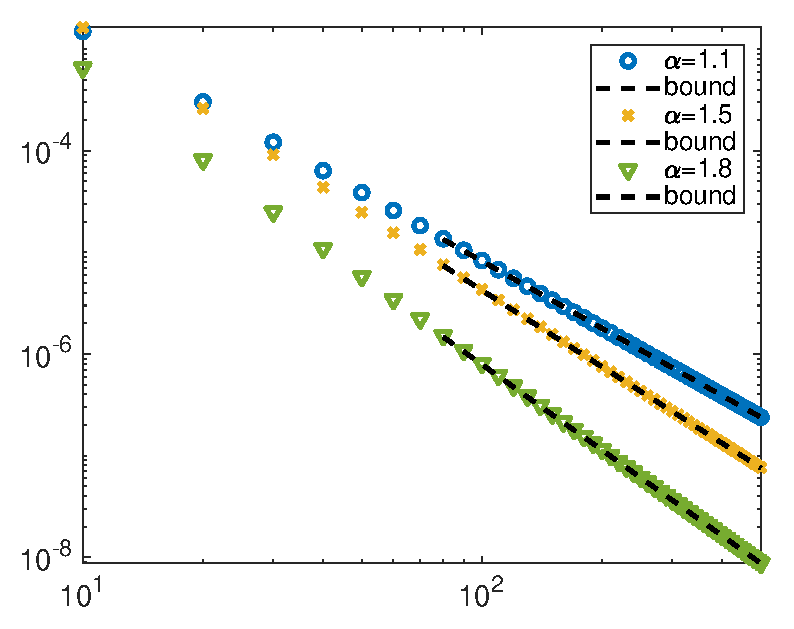
\includegraphics[width=\columnwidth]{coefbound.eps}
\end{column}
\end{columns}

	
\end{frame}

\subsection{A finite difference discretization}


\begin{frame}{A finite difference discretization}
Before going to the two-sided case in~\eqref{eq:fde1}, let us start with the simpler case
\[
\frac{\partial w}{\partial t} = - v(x) \frac{\partial w}{\partial x} + d(x) {}^{RL}D_{[0,x]}^\alpha w + f(x,t), \qquad 1 < \alpha \leq 2, \;v(x),d(x) \geq 0.
\]
\begin{enumerate}
	\item<2-> Substitute the Riemann-Liouville derivative with the \alert<2>{G}r\"unwald--\alert<2>{L}etnikov one,
	\[
	\frac{\partial w}{\partial t} = - v(x) \frac{\partial w}{\partial x} + d(x) {}^{\alert<2>{GL}}D_{[0,x]}^\alpha w + f(x,t),
	\]
	\item<3-> Choose $N \in \mathbb{N}$ at which to truncate the series expansions
	\[
	\frac{\partial w_i}{\partial t} = - v_i \frac{w_i - w_{i-1}}{h_N} + \frac{d_i}{h_N^\alpha} \sum_{k=0}^{i}(-1)^k \binom{\alpha}{k} w_{i-k} + f_i,
	\]
	\item<4-> Now we need to select a scheme for discretizing it in time: \emph{explicit}? \emph{implicit}?
\end{enumerate}
\end{frame}

\begin{frame}{A finite difference discretization: explicit Euler}
	Let us select \textbf{explicit Euler}
	\only<1-2>{\[
	\frac{w_i^{n+1} - w_i^{n}}{\Delta t} = - v_i \frac{w_i^n - w_{i-1}^n}{h_N} + \frac{d_i}{h_N^\alpha} \sum_{k=0}^{i}\only<1>{(-1)^k \binom{\alpha}{k}}\only<2->{\alert<2>{g_k}} w_{i-k}^n + f_i^n,
	\]}
	\only<3>{
	\[
	w_i^{n+1} = w_i^n - \Delta t\, v_i \frac{w_i^n - w_{i-1}^n}{h_N} + \Delta t\, \frac{d_i}{h_N^\alpha} \sum_{k=0}^{i} g_k w_{i-k}^n + f_i^n,
	\] 
	}
	\only<4-6>{
	\[
	w_i^{n+1} = \left(1 - \frac{\Delta t}{h_N} v_i + \frac{\Delta t}{h_N^\alpha} d_i \right) w_i^n + \left(\frac{v_i}{h_N} - \frac{\alpha}{h_N^\alpha} d_i\right)\Delta t w_{i-1}^n + \frac{d_i \Delta t}{h_N^\alpha} \sum_{k=2}^{i} g_k w_{i-k}^n + f_i^n \Delta t,
	\] 
	}
	\only<7-8>{
	\[
	\hat{w}_i^1 = \only<7>{\left(1 - \frac{\Delta t}{h_N} v_i + \frac{\Delta t}{h_N^\alpha} d_i \right)}\only<8->{\mu_i} \hat{w}_i^0 + \left(\frac{v_i}{h_N} - \frac{\alpha}{h_N^\alpha} d_i\right)\Delta t w_{i-1}^n + \frac{d_i \Delta t}{h_N^\alpha} \sum_{k=2}^{i} g_k w_{i-k}^n + f_i^n \Delta t,
	\]
	}
	\only<9->{
	\[
	\hat{w}_i^1 =  \mu_i \epsilon_i^0 + c_i^1,
	\]
	}
	\begin{itemize}
		\item<2-> For convenience we call $\alert<2>{g_k} = (-1)^k \binom{\alpha}{k}$,
		\item<3-> Rearrange everything to compute $w_i^{n+1}$\only<4->{, and using that $g_0 = 1$, $g_1 = -\alpha$}
		\item<5-> Is this \emph{stable}? Do we have to put a restriction on the choice of $h_N$ and $\Delta t$?
		\item<6-> Suppose that $w_i^0$ is affected by an error, i.e., $\hat{w}_i^0 = w_i^0 + \epsilon_i^0$, we can then look at the \textbf{propagation of the error},
		\item<7-> We call $\mu_i = 1 - \nicefrac{\Delta t}{h_N} v_i + \nicefrac{\Delta t}{h_N^\alpha} d_i$\only<9->{ and get the expression for the new error.}
		\item<10-> By iterating the argument we found that the error at step $n$ is amplified by the factor $\mu_i$, that is
		\[
		\epsilon_i^n = \mu_i^n \epsilon_i^0.
		\]
		\item<11-> To have stability we need to require that exist $h_N$ such that $|\mu_i|<1$ for all $h < h_N$.
	\end{itemize}
\end{frame}

\begin{frame}{A finite difference discretization: \only<1-2>{explicit}\only<3>{implicit}\only<4>{ex/implicit} Euler}
	\[
	\mu_i \equiv 1 - \frac{\Delta t}{h_N} v_i + \frac{\Delta t}{h_N^\alpha} d_i < 1 \;\Leftrightarrow\; h_N > \left(\frac{d_i}{v_i}\right)^{\nicefrac{1}{\alpha - 1}}
	\]
	\begin{itemize}
		\item[\alert{\faExclamationTriangle}] The method is not stable as $h$ is refined!
	\end{itemize}
	\begin{alertblock}<2->{Theorem~\parencite{MR2091131}}
	The \textbf{explicit} Euler solution method based on the Gr\"unwald--Letnikov approximation of the Riemann-Liouville fractional derivative is unstable.
	\end{alertblock}

	\begin{alertblock}<3->{Theorem~\parencite{MR2091131}}
	The \textbf{implicit} Euler solution method based on the Gr\"unwald--Letnikov approximation of the Riemann-Liouville fractional derivative is unstable.
	\end{alertblock}

	\only<4>{\faBriefcaseMedical\, And now what? How do we fix it?}
\end{frame}

\subsection{Shifted Gr\"unwald--Letnikov}

\begin{frame}{The Shifted Gr\"unwald--Letnikov Fractional Derivative}

\begin{exampleblock}{Shifted Gr\"unwald--Letnikov Fractional Derivative}
Let $\alpha > 0$, $f \in \mathcal{C}^{\lceil \alpha \rceil}([a,b])$, $a < x \leq b$, $\mathbb{N} \ni \alert{p} > 0$ then
\[
{}^{GL}D_{[a,x]}f(x) = \lim_{N \rightarrow + \infty} \frac{\Delta_{h_N}^\alpha f(x)}{h_N^\alpha} = \lim_{N \rightarrow + \infty} \frac{1}{h_N^\alpha}\sum_{k=0}^{N} (-1)^k \binom{\alpha}{k} f(x - (k-\alert{p}) h_N),
\]
with $h_N = (x-a)/N$.
\end{exampleblock}
\only<1-4>{If we \textbf{repeat the argument with the Fourier transform}, we discover
\[
\only<1>{\mathfrak{F}\{ {}^{GL}D_{[a,x]}f(x) \}(k) = (-ik)^\alpha \omega( -ikh ) \hat{f}(k),}
\only<2>{\mathfrak{F}\{ {}^{GL}D_{[a,x]}f(x) \}(k) = (-ik)^\alpha \hat{f}(k) + (ik)^{\alpha} (\omega(-ikh) - 1)\hat{f}(k) }
\only<3->{\mathfrak{F}\{ {}^{GL}D_{[a,x]}f(x) \}(k) = \mathcal{F}\{ {}^{RL}D_{(-\infty,x]}^\alpha f\}(k) + \hat{\phi}(k,h)  }
\]
with
\only<1-3>{\[
\omega(z) = \left(\frac{1 - e^{-z}}{z}\right)^\alpha e^{zp} = 1 - \left(p-\frac{\alpha}{2}\right)z + O(|z|^2)\only<2->{ \Rightarrow\, |\omega(-ix)-1| \leq C x \, \forall\,x \in \mathbb{R}}.
\]}
\only<4>{
\[
|\phi(k,h)| \leq |k|^\alpha C|hk| |\hat{f}(k)|\,\Rightarrow\, |\phi(h,x)| < I C h, \quad I = \int_{-\infty}^{+\infty} (1+|k|)^{\alpha+1} |\hat{f}(k)|\,\mathrm{d}k < +\infty.
\]
}}
\only<5->{
\begin{itemize}
	\item<5-> They give the same operator uniformly in $x$ as $h \rightarrow 0$, therefore we can use the shifted version with \emph{any} shift to approximate the Riemann-Liouville derivative,
	\item<6-> To get the \emph{best constant} $C$ we can minimize the $|p-\nicefrac{\alpha}{2}|$ term in $\omega(z)$, that is, we select $p = 1$.
	\item[\faQuestionCircle]<7-> Let us see if using the \emph{shifted version} with $p = 1$ solves our \textbf{stability problem}.
\end{itemize}
}
\end{frame}

\begin{frame}{Back to finite differences: implicit Euler}

We use the \textbf{shifted Gr\"unwald--Letnikov} and the \textbf{implicit Euler} method
\only<1>{\[
\frac{w_i^{n+1} - w_i^n}{\Delta t} = - v_i \frac{w_i^{n+1} - w_{i-1}^{n+1}}{h_N} + \frac{d_i}{h_N^\alpha} \sum_{k=0}^{i+1} g_k w_{i-k+1}^{n+1} + f_{i}^{n+1}.
\]}
\only<2>{\[
w_i^{n+1} - w_i^n = - \alert{E_i} (w_i^{n+1} - w_{i-1}^{n+1}) + \textcolor{blue}{B_i} \sum_{k=0}^{i+1} g_k w_{i-k+1}^{n+1} + \Delta t f_{i}^{n+1}.
\]}
\only<3->{
\[
-g_0 B_i w_{i+1}^{n+1} + (1+E_i -g_i B_i) w_i^{n+1} - (E_i + g_2 B_i) w_{i-1}^{n+1} - B_{i} \sum_{k=3}^{i+1} g_k w_{i-k+1}^{n+1} = c_i^n + \Delta t \, f_i^{n+1}.
\]
}
\begin{columns}
\begin{column}{0.3\columnwidth}
	\begin{itemize}
		\item<2-> Set $\alert{E_i} = \nicefrac{v_i \Delta t}{h_N}$, $\textcolor{blue}{B_i} = \nicefrac{d_i \Delta t}{h_N^\alpha}$, 
		\item<3-> reorder the system of equations,
		\item<4-> and obtain
		\[
		\hspace{-1.5em} \alert<5>{A_N} \mathbf{w}^{n+1} = \mathbf{w}^n + \Delta t\,\mathbf{f}^{n+1}.
		\]
	\end{itemize}
\end{column}	
\begin{column}{0.7\columnwidth}\small
\only<5>{\[\hspace{-1.5em}
\begin{bmatrix}
	1 & 0  & 0 & \cdots & \cdots & 0\\
-E_1 - g_2 B_1 & 1 + E_1 -g_1 B_1	 & -g_0 B_1 & \ddots \\
-g_3 B_2 & -E_2 - g_2 B_2 & 1 + E_2 -g_1 B_2	 & -g_0 B_2 & \ddots \\
\vdots & \ddots & \ddots & \ddots & \ddots & \vdots \\
-g_N B_{N-1} & \cdots & \cdots & \cdots & \cdots & - g_0 B_{N-1} \\
0 & \cdots & \cdots & \cdots & \cdots & 1 
\end{bmatrix}
\]}
\only<6->{\[
\begin{split}
{\mathbf{w}^{n+1}} = & [w_0^{n+1},w_1^{n+1},\ldots,w^{n+1}_N]^T,\\
{\mathbf{w}^{n}} = & [w_0^{n},w_1^{n},\ldots,w^{n}_N]^T,\\
\mathbf{f}^{n+1} = & \Delta t [0,f_1^n,\ldots,f_{N-1}^n,0]^T.
\end{split}
\]

\onslide<7>{\centering \faWrench\;To prove \textbf{stability} we need to have $\rho(A_N^{-1}) \leq 1$: \[\boldsymbol{\epsilon}^1 = A_N^{-1} \boldsymbol{\epsilon}^0. \]}
}
\end{column}
\end{columns}


\end{frame}

\begin{frame}{Back to finite differences: implicit Euler}

Let $(\lambda,\mathbf{x})$ be an eigencouple of $A_N$, i.e., $A_N \mathbf{x} = \lambda \mathbf{x}$, $\mathbf{x} \neq \mathbf{0}$.
\begin{enumerate}
	\item<2-> Choose $i$ such that $|x_i| = \max\{ |x_j| \,:\; j=0,\ldots,N \}$,
	\item<3-> Then $\displaystyle \sum_{j=0}^{N} (A_N)_{i,j} x_j = x_i$, and thus
	\[
	\lambda = A_{i,i} + \sum_{\substack{j=0\\j\neq i}}^N (A_N)_{i,j} \frac{x_j}{x_i},
	\] 
	\item<4-> If $i = 0$ or $i = N$ then $\lambda = 1$, otherwise
	\only<4>{\[
	\lambda = 1 + E_i - g_1 B_1 - g_0 B_i \frac{x_{i+1}}{x_i}  (E_i + g_2 B_i) \frac{x_{i-1}}{x_i} - B_i \sum_{j=0}^{i-2} h_{i-j+1} \frac{x_j}{x_i}
	\]}
	\only<5>{
	\[
	\lambda = 1 + E_i(1 - \nicefrac{x_{i-1}}{x_i}) - B_i \left[ g_1 + \sum_{\substack{j=0\\j\neq i}}^{i+1} g_{i-j+1} \frac{x_j}{x_i} \right]
	\]
	}
\end{enumerate}

\end{frame}

\begin{frame}{Back to finite differences: implicit Euler}
	\begin{enumerate}
	\setcounter{enumi}{3}
	\item We have $\sum_{k \geq 0} g_k = 0$, $\alpha \in (1,2]$ and thus $g_1 = -\alpha$ and $g_k \geq 0$ for $k \neq 1$, thus
	\[
	-g_1 \geq \sum_{\substack{k=0\\k\neq 1}}^j g_k \qquad \forall\,j=0,1,2,\ldots
	\]
	furthermore $|\nicefrac{x_j}{x_i}| < 1$, and thus
	\[
	\sum_{\substack{j=0\\j\neq i}}^{i+1} g_{i-j+1} \left|\frac{x_j}{x_i}\right| \leq \sum_{\substack{j=0\\j\neq i}}^{i+1} g_{i-j+1} \leq - g_1.
	\]
	\setcounter{enumi}{2}
	\item<2-> If $i = 0$ or $i = N$ then $\lambda = 1$, otherwise
	\[
		|\lambda| \geq 1 + \underbrace{E_i}_{\geq 0}(1 - \underbrace{\nicefrac{x_{i-1}}{x_i}}_{\leq 1}) + \underbrace{B_i}_{\geq 0} \left[ g_1 + \sum_{\substack{j=0\\j\neq i}}^{i+1} g_{i-j+1} \left|\frac{x_j}{x_i}\right| \right] \geq 1.
	\]
	\end{enumerate}

\end{frame}

\begin{frame}{Back to finite differences: implicit Euler}
	\begin{alertblock}{Theorem \parencite{MR2091131}}
	The implicit Euler method solution to
	\[
	\frac{\partial w}{\partial t} = - v(x) \frac{\partial w}{\partial x} + d(x) {}^{RL}D_{[0,x]}^\alpha w + f(x,t), \qquad 1 < \alpha \leq 2, \;v(x),d(x) \geq 0.
	\]
	with boundary conditions $w(0,t) = 0$, $w(1,t) = 0$ for all $t \geq 0$, based on the shifted Gr\"unwald--Letnikov approximation with $h_N = 1/N$, is consistent
	of order $O(h + \Delta t)$ and \emph{unconditionally stable}.
	
	\end{alertblock}
\begin{itemize}
	\item[\faEye] We have only a left-sided fractional derivative, we could put a non-homogeneous condition on the right-hand side,
	\item[\faMagic] We can now start \textbf{looking into the matrices} to devise solution strategies for the \emph{sequence of linear systems}
	\[
	A_N \mathbf{w}^{n+1} = \mathbf{w}^n + \Delta t\,\mathbf{f}^{n+1}.
	\]  
\end{itemize}
\end{frame}

\subsection{Gr\"unwald--Letnikov matrices}

\begin{frame}{Gr\"unwald--Letnikov matrices}
To look at the matrices we go back to the first form of the diffusion equation~\eqref{eq:fde1}
	\begin{equation*}
	\begin{cases}\frac{\partial W}{\partial t} = \theta\,{}^{\only<1>{RL}\only<2->{\alert<2>{GL}}}D_{[0,x]}^\alpha W(x,t) + (1-\theta) {}^{\only<1>{RL}\only<2->{\alert<2>{GL}}}D_{[x,1]}^\alpha W(x,t), \qquad \theta \in [0,1],\\
	W(0,t) = W(1,t) = 0,\\
	W(x,t) = W_0(x).	
	\end{cases}
	\end{equation*}
\begin{enumerate}
	\item<2-> Substitute the Riemann-Liouville derivative with the \alert<2>{G}r\"unwald--\alert<2>{L}etnikov one,
	\item<3-> Choose $N \in \mathbb{N}$ at which to truncate the \emph{shifted} series expansions
	\only<3>{\[
	h_N^\alpha \, \frac{\partial W_{i}}{\partial t} = \theta \sum_{k=0}^{i+1} (-1)^k \binom{\alpha}{k} W_{i-k+1} + (1-\theta)  \sum_{k=0}^{N-i+2} (-1)^k \binom{\alpha}{k} W_{i+k-1}, \; i=0,\ldots,N.
	\]}
	\item<4-> Apply, e.g., \emph{backward Euler} to discretize the derivative w.r.t. time
	\only<4>{
	\[
	\hspace{-3.2em}\frac{h_N^\alpha}{\Delta t} (W_{i}^{j+1} - W_i^{j}) = \theta \sum_{k=0}^{i-k+1} (-1)^k \binom{\alpha}{k} W_{i-k+1}^{j} + (1-\theta)  \sum_{k=0}^{N+i-2} (-1)^k \binom{\alpha}{k} W_{i+k-1}^j, \begin{array}{l}i=0,\ldots,N,\\j=0,\ldots,M-1.\end{array}
	\]
	}
\end{enumerate}
\end{frame}



\begin{frame}[fragile]{The matrix formulation}

We call again $\mathbf{w}^{j}$, $\mathbf{w}^{j+1}$ the vectors containing the solution \textbf{on inner grid points}, then we can rewrite the set of linear equations as
\[
\left( I_N - \frac{\Delta t}{h_N^\alpha} \left[ \theta G_N + (1-\theta) G_N^T \right] \right) \mathbf{w}^{n+1} = \mathbf{w}^n
\]
where
\begin{columns}
\begin{column}{0.4\columnwidth}
\[
G_N = \begin{bmatrix}
	1 & 0 & \cdots & \cdots & 0 \\
	g_2 & g_1 & g_0 \\
	\vdots & \ddots & \ddots & \ddots\\
	\vdots &  & \ddots &  \ddots & g_0 \\
	g_{N-1} & \cdots & g_3 & g_2 & g_1 \\
	0 & \cdots & \cdots & 0 & 1
\end{bmatrix}
\]
\end{column}
\begin{column}{0.6\columnwidth}
\definecolor{bg}{rgb}{0.95,0.95,0.95}
\begin{minted}[bgcolor=bg,fontsize=\small,breaklines]{matlab}
function G = glmatrix(N,alpha)
%%GLMATRIX produces the GL discretization of  
% the Riemann-Liouville derivative
g = gl(N,alpha);
c = zeros(N,1); r = zeros(1,N);
r(1:2) = g(2:-1:1); 
c(1:N) = g(2:end);
G = toeplitz(c,r);
end
\end{minted}
\end{column}
\end{columns}
\end{frame}

\begin{frame}[fragile]{The matrix formulation}
To obtain a simple code for the complete problem
\begin{columns}
\begin{column}{0.6\columnwidth}
\definecolor{bg}{rgb}{0.95,0.95,0.95}
\begin{minted}[bgcolor=bg,fontsize=\small,breaklines]{matlab}
%% Discretization data
hN = 1/(N-1); x = 0:hN:1;
dt = hN; t = 0:dt:1;
%% Discretize
G = glmatrix(N,alpha); Gt = glmatrix(N,alpha).';
I = eye(N,N);
% apply B.C.
G(1,:) = -I(1,:); G(N,:) = -I(N,:);
Gt(1,:) = -I(1,:); Gt(N,:) = -I(N,:);
% Left-hand side
A = I - dt/hN^alpha*(theta*G + (1-theta)*Gt);
% Right-hand side
w = w0(x).'; 
\end{minted}
\end{column}
\begin{column}{0.4\columnwidth}
\begin{itemize}
\item Select $\theta = \nicefrac{1}{2}$, $\alpha = \nicefrac{3}{2}$, and $W_0(x) = 5 x(1-x)$,
\item Discretize the interval $[0,1]$ on $N$ points,
\item Build the $I$ and $G_N$ matrices,
\item Apply the Dirichlet b.c.s,
\item Assemble $A$ and $\mathbf{w}^0$.
\end{itemize}

\begin{onlyenv}<2->
March the scheme in time:
\definecolor{bg}{rgb}{0.95,0.95,0.95}
\begin{minted}[bgcolor=bg,fontsize=\small,breaklines]{matlab}
for i=2:N
  w = A\w;
end
\end{minted}
\end{onlyenv}

\end{column}
\end{columns}

\end{frame}

\begin{frame}
\begin{columns}
\begin{column}{0.33\columnwidth}
\centering	
	
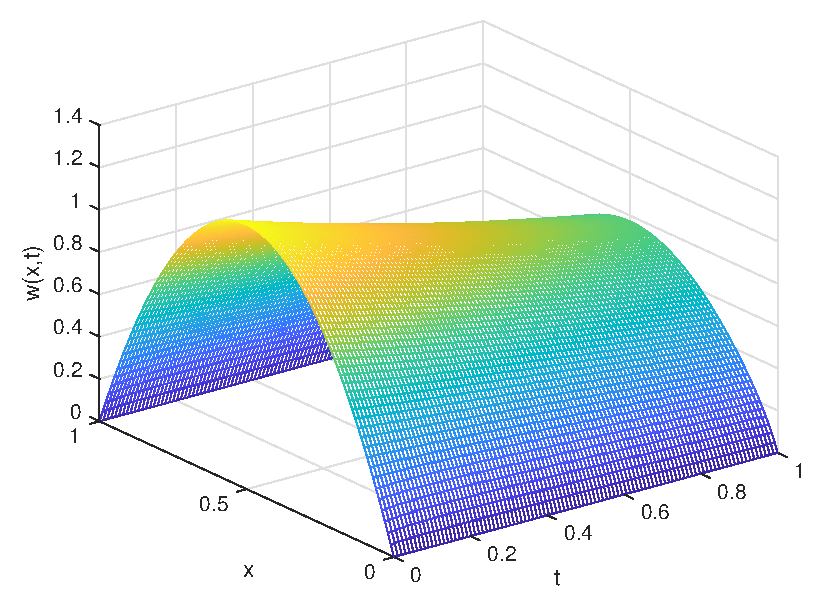
\includegraphics[width=\columnwidth]{sol_alpha11.eps}

$\alpha = 1.1$, $\theta = 0.5$
\end{column}
\begin{column}{0.33\columnwidth}
\centering	

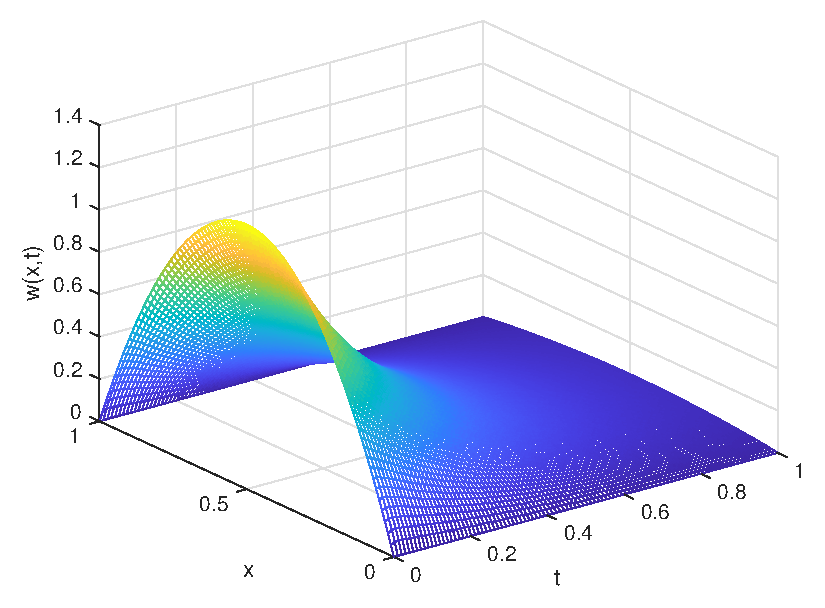
\includegraphics[width=\columnwidth]{sol_alpha15.eps}
 
$\alpha = 1.5$, $\theta = 0.5$
\end{column}
\begin{column}{0.33\columnwidth}
\centering	

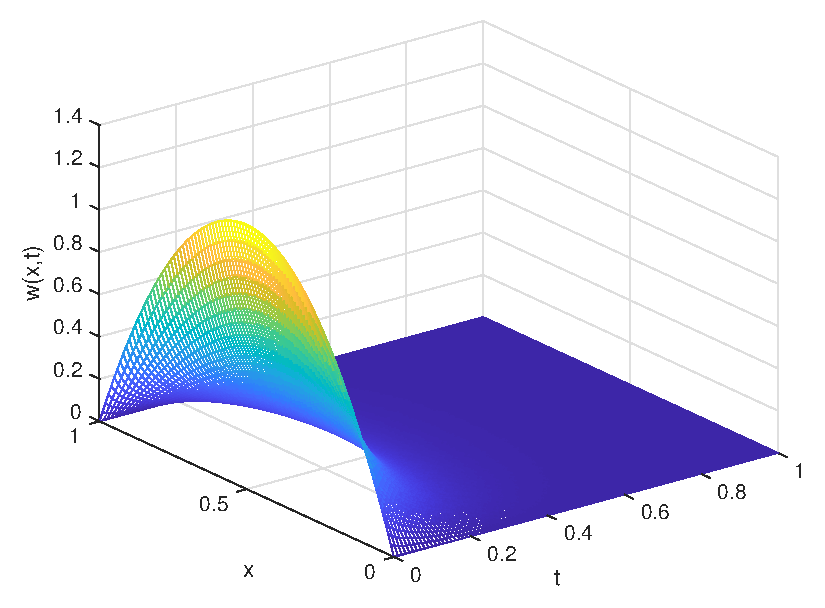
\includegraphics[width=\columnwidth]{sol_alpha20.eps}

$\alpha = 2.0$, $\theta = 0.5$
\end{column}
\end{columns}

\begin{columns}
\begin{column}{0.33\columnwidth}
	\centering	
	
	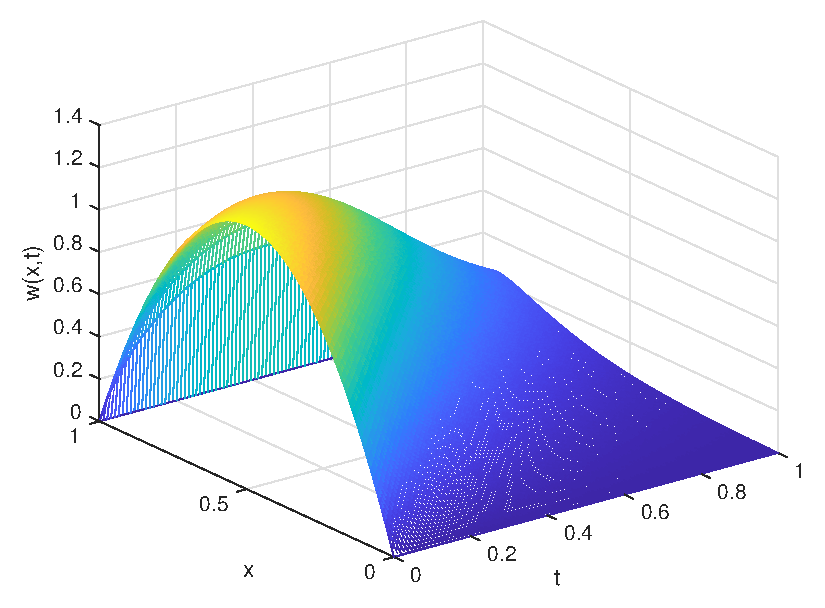
\includegraphics[width=\columnwidth]{sol_alpha11_skew.eps}
	
	$\alpha = 1.1$, $\theta = 0.1$
\end{column}
\begin{column}{0.33\columnwidth}
	\centering	
	
	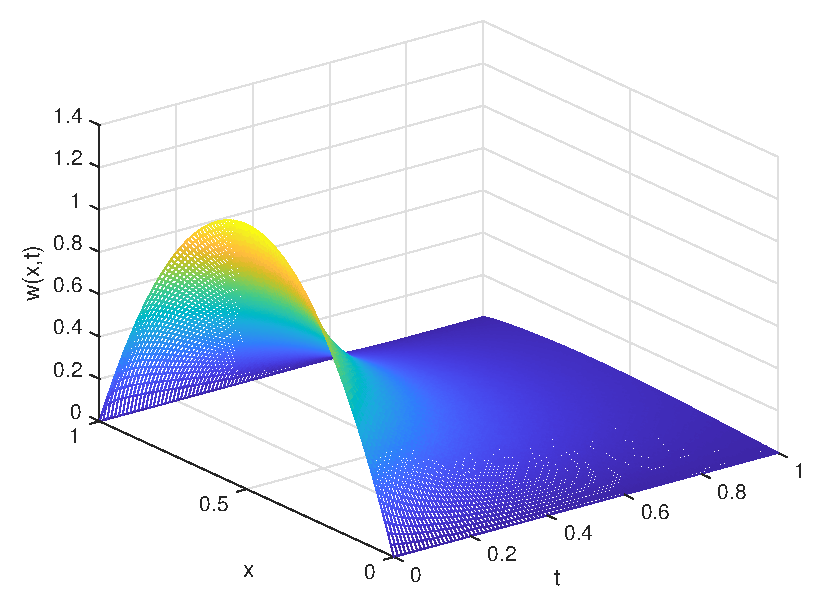
\includegraphics[width=\columnwidth]{sol_alpha15_skew.eps}
	
	$\alpha = 1.5$, $\theta = 0.3$
\end{column}
\begin{column}{0.33\columnwidth}
	\centering	
	
	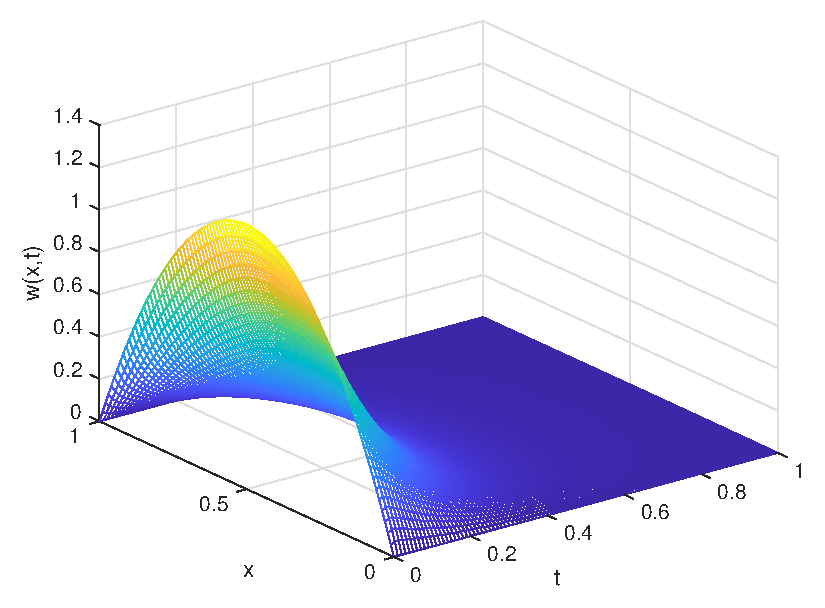
\includegraphics[width=\columnwidth]{sol_alpha18_skew.eps}
	
	$\alpha = 1.8$, $\theta = 0.9$
\end{column}
\end{columns}

\end{frame}

\begin{frame}{The solution step}

\begin{itemize}
	\item[\faQuestionCircle] How can we \textbf{efficiently solve} the linear systems
	\[
	A \mathbf{w}^{n+1} = \mathbf{w}^n,
	\]
	needed for the time-stepping?
	\item[\faQuestionCircle] Can we find a reliable procedure working also for \textbf{multi-dimensional cases}?
	\item[\faQuestionCircle] Is \textbf{dense linear algebra} a compulsory choice?
	
	\begin{columns}
	\begin{column}{0.6\columnwidth}
	\onslide<2>{
	\Large\centering
	
	These matrices have \alert{structure\textbf{s}} we can \textbf{exploit}!}
	\end{column}
	\begin{column}{0.4\columnwidth}
	\onslide<2>{
	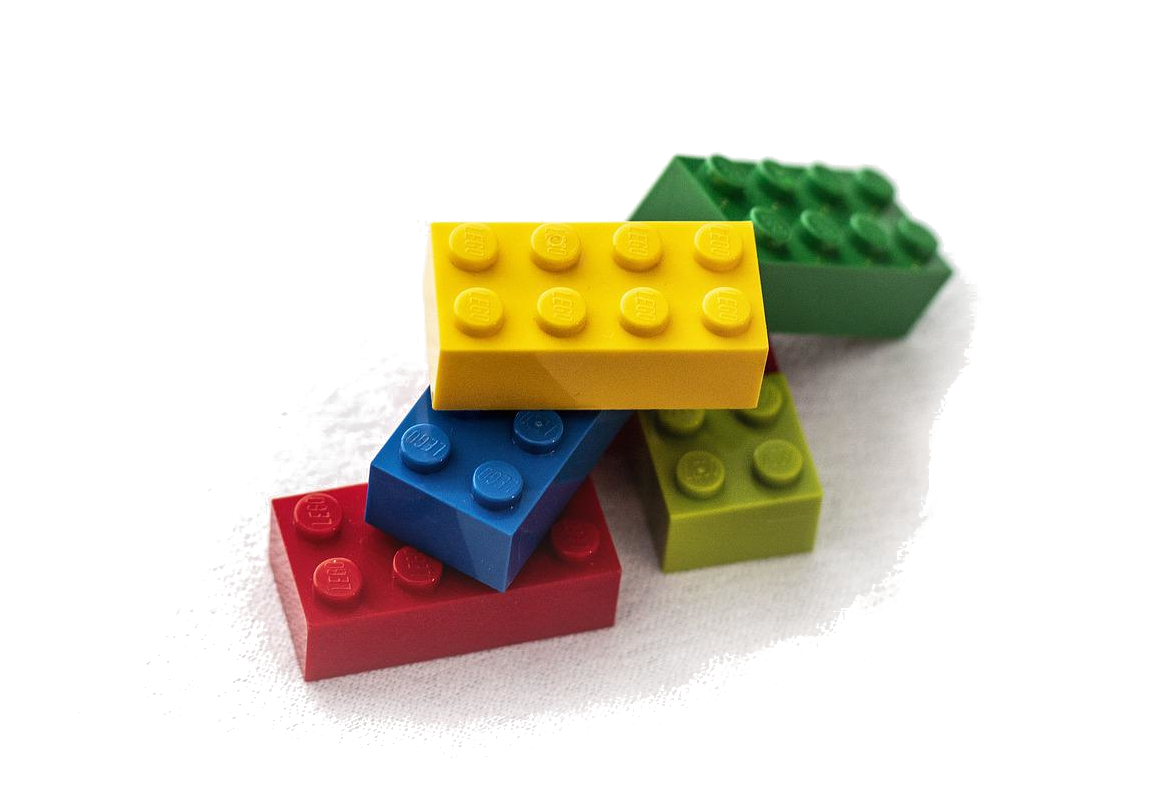
\includegraphics[width=\columnwidth]{costruzioni.png}
	}
	\end{column}
	\end{columns}
\end{itemize}

\end{frame}


\begin{frame}{Toeplitz matrices}\vspace{-0.5em}

\begin{block}{Toeplitz matrix}
A \textbf{Toeplitz matrix} is a matrix whose entries are constant along the diagonals
\begin{equation*}
	T_n(f) = \begin{bmatrix}
		t_0 & t_{-1} & \ldots & t_{2-n} & t_{1-n} \\
		t_{1} & t_0 & t_{-1} & \ldots & t_{2-n}  \\
		\vdots & t_1 & t_0 & \ddots &  \vdots \\
		t_{n-2} & \ldots & \ddots & \ddots & t_{-1} \\
		t_{n-1} & t_{n-2} & \ldots & t_1 & t_0
	\end{bmatrix}.
\end{equation*}
\end{block}

\begin{block}<2>{Generating function}
$$
f(x) = \sum_{k = -\infty}^{+\infty} t_k e^{i\cdot kx}, \quad t_k
=\frac{1}{2\pi}\int_{-\pi}^{\pi} f(\theta) e^{-ik\theta}d\theta, \
k=0,\pm 1, \pm 2, \ldots
$$
the $t_k$ are the Fourier coefficients is called
a \textit{generating function} of the matrix $T_n(f)$.
\end{block}

\end{frame}

\begin{frame}{Circulant matrices}
	\begin{block}{Circulant matrix}
		A \textbf{Circulant matrix} $C_n \in \mathbb{R}^{n\times n}$ is a
		Toeplitz matrix in which each row is a cyclic shift of the row above it, i.e.,
		$(C_n)_{i,j} = c_{(j-i)\mod{n}}$:
		\begin{equation*}
			C_n = \begin{bmatrix}
				c_0 & c_1 & c_2 & \ldots & \ldots & c_{n-1} \\
				c_{n-1} & c_0 & c_1 & \ddots & & \vdots \\
				c_{n-2} & c_{n-1} & c_0 & c_1 & \ddots & \vdots \\
				\vdots & \ddots & \ddots & \ddots & \ddots & c_2 \\
				\vdots &  & \ddots & \ddots & c_0 & c_1 \\
				c_1 & \ldots & \ldots & c_{n-2} & c_{n-1} & c_0
			\end{bmatrix}.
		\end{equation*}
	\end{block}
\end{frame}

\begin{frame}{Toeplitz and Circulant matrices: some properties}
\begin{alertblock}{Properties}
\begin{enumerate}
	\item The operator $T_n : \mathbb{L}^1[-\pi,\pi] \rightarrow
	\mathbb{C}^{n\times n}$ defined by the Toeplitz matrix construction is linear and positive, i.e., if $f \geq 0$ then $T_n(f) = T_n(f)^H$
	$\forall \, n$ and $\mathbf{x}^H T_n(f)
	\mathbf{x} \geq 0$ $\forall \, \mathbf{x} \in \mathbb{C}^{n}$.
	\item Given $f \in \mathbb{L}^{1}[-\pi,\pi]$ such that $m_f =
	\operatorname{ess}\inf(f)$ and $M_f = \operatorname{ess}\sup(f)$. 
	
	If $m_f > -\infty$ then $m_f \leq \lambda_j(T_n(f))$ $\forall
	j=1,\ldots,n$;
	
	If $M_f < \infty$ then $M_f \geq \lambda_j(T_n(f))$
	$\forall j=1,\ldots,n$. 
	
	If $f$ is not identical to a real
	constant and both the inequalities hold,
	\begin{equation*}
		m_f < \lambda_j(T_n(f)) < M_f \;\; \forall j=1,\ldots,n.
	\end{equation*}
	
	\item Circulant matrices are simultaneously diagonalized by the unitary matrix $F_n$
	\begin{equation*}
		\left(F_n\right)_{j,k}=\frac{1}{\sqrt{n}}e^{\frac{-2\pi i\, j\,
			k}{n}}, \mathcal{C} = \left\lbrace C_n\in \mathbb{C}^{n\times n} \mid C_n=F D F^H \;:\; D =
		\operatorname{diag}(d_0,d_1,\ldots,d_{n-1}) \right\rbrace.
	\end{equation*}
\end{enumerate}
\end{alertblock}
\end{frame}



\begin{frame}{Asymptotic distribution - I}
\begin{block}{Asymptotic eigenvalue distribution}
Given a sequence of matrices
$\{X_n\}_n \in \mathbb{C}^{d_n\times d_n}$
with $d_n = \{\dim X_n\}_n \overset{ n \rightarrow
	+\infty}{\longrightarrow} \infty$ monotonically and a
$\mu$-measurable function $f : D \rightarrow \mathbb{R}$, with
$\mu(D) \in (0,\infty)$, we say that the sequence $\{X\}_n$ is
distributed  in the sense of the eigenvalues as the function $f$ and
write $\{X_n\}_n \sim_{\lambda} f$ if and only if,
\begin{equation*}
	\lim_{n \rightarrow \infty} \frac{1}{d_n} \sum_{j = 0}^{d_n}
	F(\lambda_j(X_n)) = \frac{1}{\mu(D)} \int_{D}F(f(t))dt, \;\; \forall
	\, F \in \mathcal{C}_c(D),
\end{equation*}
where $\lambda_j(\cdot)$ indicates the $j$-th eigenvalue.
\end{block}
\end{frame}

\begin{frame}{Asymptotic distribution - II}

\begin{block}{Asymptotic singular value distribution}
    Given a sequence of matrices $\{X_n\}_n \in \mathbb{C}^{d_n \times
	d_n}$
with $d_n = \{\dim X_n\}_n \overset{ n \rightarrow
	+\infty}{\longrightarrow} \infty$ monotonically and a $\mu$-measurable
function $f : D \rightarrow \mathbb{R}$, with $\mu(D) \in (0,\infty)$,
we say that the sequence $\{X\}_n$ is distributed
in the sense of the singular values as the function $f$ and write
$\{X_n\}_n \sim_{\sigma} f$ if and only if
\begin{equation*}
	\lim_{n \rightarrow \infty} \frac{1}{d_n} \sum_{j = 0}^{d_n}
	F(\sigma_j(X_n)) = \frac{1}{\mu(D)} \int_{D}F(|f(t)|)dt, \;\; \forall
	\, F \in \mathcal{C}_c(D),
\end{equation*}
where $\sigma_j(\cdot)$ is the $j$-th singular value.
\end{block}

\end{frame}

\begin{frame}{Asymptotic distribution - III}

\begin{alertblock}{Theorem (Asymptotic distribution of Toeplitz matrices)}
Given the generating function $f$, $T_n(f)$ is distributed in the sense of
the eigenvalues as $f$, written also as $T_n(f)
\sim_{\lambda} f$, if one of the following conditions hold:
\begin{enumerate}
	\item~\parencite{grenander2001toeplitz}: $f$ is real valued and $f
	\in \mathbb{L}^{\infty}$,
	\item~\parencite{tyrtyshnikov1996unifying}: $f$ is real valued and $f
	\in \mathbb{L}^{2}$.
\end{enumerate}
Moreover, $T_n(f)$ is distributed in the sense of
the singular values as $f$, written also as
$T_n(f) \sim_{\sigma} f$, if one of the following conditions
hold:
\begin{enumerate}
	\item~\parencite{avram1988bilinear,parter1986distribution}: $f \in
	\mathbb{L}^{\infty}$,
	\item~\parencite{tyrtyshnikov1996unifying}: $f \in \mathbb{L}^{2}$.
\end{enumerate}
\end{alertblock}

\end{frame}

\begin{frame}[fragile]{Singular value distribution of $G_N$}

\begin{itemize}
	\item[\faPuzzlePiece]<1-> The matrix $G_N$ is a \textbf{Toeplitz} and \textbf{Hessenberg} matrix,
	\item[\faQuestionCircle]<2-> Does it have a \textbf{generating function}?
	\item<3-> \alert{\textbf{Yes}!} And we have already computed it several times! The coefficients $\{g_k^{(\alpha)}\}_k$ where given by the \textbf{binomial expansion} of $(1+z)^\alpha$, and thus
	\[
	f(\theta) = e^{-i \theta} \left(1 + \exp(i(\theta+\pi))\right)^\alpha, \qquad \theta \in [0,2\pi)
	\]
\end{itemize}\vspace{-1.5em}
\begin{columns}
\begin{column}{0.5\columnwidth}
\begin{onlyenv}<4->%
\vspace{-0.5em}\definecolor{bg}{rgb}{0.95,0.95,0.95}
\begin{minted}[bgcolor=bg,fontsize=\small,breaklines]{matlab}
N = 100;
alpha = 1.5;
G = glmatrix(N,alpha);
s = @(t) exp(-1i*t).*(1 + ...
 exp(1i*(t+pi))).^alpha; 
sv = svd(G);
th = linspace(0,2*pi,N);
plot(th,sv,'o',th,sort(abs(s(th)),...
 'descend'),'-','LineWidth',2);
\end{minted}
\end{onlyenv}
\end{column}
\begin{column}{0.5\columnwidth}
\only<4>{
\centering

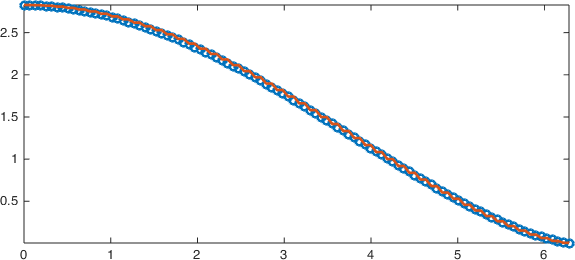
\includegraphics[width=\columnwidth]{svd.png}

}
\end{column}
\end{columns}


\end{frame}

\section{Conclusion and summary}

\begin{frame}{Conclusion and summary}
\definecolor{success}{HTML}{4a934a}
\definecolor{todo}{HTML}{0099cc}

\begin{itemize}
	\item[\textcolor{success}{\faCheckCircle}] We introduced \textbf{p}artial \textbf{d}ifferential \textbf{e}quations with \textbf{f}ractional (FPDE) derivative with respect to the space variables,
	\item[\textcolor{success}{\faCheckCircle}] we connected \emph{fractional diffusion} and continuous time random walk using \emph{L\'evy flights},
	\item[\textcolor{success}{\faCheckCircle}] we introduced the Gr\"unwald-Letnikov fractional derivative, highlighted the connection with the Riemann-Liouville derivative.
	\item[\textcolor{success}{\faCheckCircle}] We introduced a \emph{stable discretization} of finite difference type,
	\item[\textcolor{success}{\faCheckCircle}] and we started investigating the structure of the underlying matrices.
\end{itemize}

Next up
\begin{itemize}
	\item[\textcolor{todo}{\faClipboardList}] Investigating the structure of the underlying matrices for different FPDEs.
	\item[\textcolor{todo}{\faClipboardList}] Looking into some preconditioners and solution strategies based on structured matrices.
\end{itemize}

\end{frame}

\appendix

\section*{Bibliography}
{\unnumbered
	\begin{frame}[allowframebreaks,noframenumbering]{Bibliography}
	\small
	\printbibliography
	
\end{frame}
}

\end{document}